%%
%% This is file `sample-manuscript.tex',
%% generated with the docstrip utility.
%%
%% The original source files were:
%%
%% samples.dtx  (with options: `all,proceedings,bibtex,manuscript')
%% 
%% IMPORTANT NOTICE:
%% 
%% For the copyright see the source file.
%% 
%% Any modified versions of this file must be renamed
%% with new filenames distinct from sample-manuscript.tex.
%% 
%% For distribution of the original source see the terms
%% for copying and modification in the file samples.dtx.
%% 
%% This generated file may be distributed as long as the
%% original source files, as listed above, are part of the
%% same distribution. (The sources need not necessarily be
%% in the same archive or directory.)
%%
%%
%% Commands for TeXCount
%TC:macro \cite [option:text,text]
%TC:macro \citep [option:text,text]
%TC:macro \citet [option:text,text]
%TC:envir table 0 1
%TC:envir table* 0 1
%TC:envir tabular [ignore] word
%TC:envir displaymath 0 word
%TC:envir math 0 word
%TC:envir comment 0 0
%%
%% The first command in your LaTeX source must be the \documentclass
%% command.
%%
%% For submission and review of your manuscript please change the
%% command to \documentclass[manuscript, screen, review]{acmart}.
%%
%% When submitting camera ready or to TAPS, please change the command
%% to \documentclass[sigconf]{acmart} or whichever template is required
%% for your publication.
%%
%%
\documentclass[manuscript,screen,review]{acmart}
%%
%% \BibTeX command to typeset BibTeX logo in the docs

\usepackage{geometry}
\usepackage{todonotes}
\usepackage{setspace}
\usepackage{caption}
\usepackage{graphicx}
\usepackage{url}
\usepackage{multirow}
% \usepackage{amsmath}%, amsmath}%, amssymb}
% \usepackage{mathptmx}
\usepackage[T1]{fontenc}
\usepackage{natbib}
\usepackage{listings}
\usepackage[utf8x]{inputenc}




\newcommand{\ME}{\mathcal{E}}
\newcommand{\MA}{\mathcal{A}}
\newcommand{\MW}{\mathcal{W}}
\newcommand{\MT}{\mathcal{T}}
\newcommand{\MC}{\mathcal{C}}
\newcommand{\MD}{\mathcal{V}}
\newcommand{\MN}{\mathcal{N}}
\newcommand{\MP}{\mathcal{P}}
\newcommand{\MV}{\mathcal{V}}
\newcommand{\MX}{\mathcal{X}}
\newcommand{\MH}{\mathcal{H}}
\newcommand{\ML}{\mathcal{L}}
\newcommand{\MI}{\mathcal{I}}
\newcommand{\MK}{\mathcal{K}}
\newcommand{\MY}{\mathcal{Y}}
\newcommand{\BB}{\mathbb{B}}
\newcommand{\R}{\mathbb{R}}
\newcommand{\NN}{\mathbb{N}}
\newcommand{\predict}{\mathcal{P}}
\newcommand{\RR}{\mathbb{R}}
\newcommand{\MZ}{\mathcal{Z}}
\newcommand{\MS}{\mathcal{S}}
\newcommand{\unif}{\pazocal{U}}
\newcommand{\mysum}{\displaystyle \sum_{i=1}^n}
% \AtBeginDocument{%
%   \providecommand\BibTeX{{%
%     Bib\TeX}}}

%% Rights management information.  This information is sent to you
%% when you complete the rights form.  These commands have SAMPLE
%% values in them; it is your responsibility as an author to replace
%% the commands and values with those provided to you when you
%% complete the rights form.
% \setcopyright{acmlicensed}
% \copyrightyear{2018}
% \acmYear{2018}
% \acmDOI{XXXXXXX.XXXXXXX}
%% These commands are for a PROCEEDINGS abstract or paper.
% \acmConference[Conference acronym 'XX]{Make sure to enter the correct
%   conference title from your rights confirmation email}{June 03--05,
%   2018}{Woodstock, NY}
%%
%%  Uncomment \acmBooktitle if the title of the proceedings is different
%%  from “Proceedings of ...''!
%%
%%\acmBooktitle{Woodstock '18: ACM Symposium on Neural Gaze Detection,
%%  June 03--05, 2018, Woodstock, NY}
% \acmISBN{978-1-4503-XXXX-X/2018/06}


%%
%% Submission ID.
%% Use this when submitting an article to a sponsored event. You'll
%% receive a unique submission ID from the organizers
%% of the event, and this ID should be used as the parameter to this command.
%%\acmSubmissionID{123-A56-BU3}

%%
%% For managing citations, it is recommended to use bibliography
%% files in BibTeX format.
%%
%% You can then either use BibTeX with the ACM-Reference-Format style,
%% or BibLaTeX with the acmnumeric or acmauthoryear sytles, that include
%% support for advanced citation of software artefact from the
%% biblatex-software package, also separately available on CTAN.
%%
%% Look at the sample-*-biblatex.tex files for templates showcasing
%% the biblatex styles.
%%

%%
%% The majority of ACM publications use numbered citations and
%% references.  The command \citestyle{authoryear} switches to the
%% "author year" style.
%%
%% If you are preparing content for an event
%% sponsored by ACM SIGGRAPH, you must use the "author year" style of
%% citations and references.
%% Uncommenting
%% the next command will enable that style.
%%\citestyle{acmauthoryear}


%%
%% end of the preamble, start of the body of the document source.
\begin{document}

%%
%% The "title" command has an optional parameter,
%% allowing the author to define a "short title" to be used in page headers.
\title{Exploring LLM Features in Predictive Process Monitoring for Small-Scale Event-Logs}

%%
%% The "author" command and its associated commands are used to define
%% the authors and their affiliations.
%% Of note is the shared affiliation of the first two authors, and the
%% "authornote" and "authornotemark" commands
%% used to denote shared contribution to the research.
\author{Alessandro Padella}
\email{alessandro.padella@unipd.it}
\orcid{0009-0008-6399-9364}
\affiliation{%
  \institution{Università degli Studi di Padova}
  \city{Padova}
  \country{Italy}
}

\author{Massimiliano de Leoni}\orcid{0000-0002-8447-5374}
\affiliation{%
  \institution{Università degli Studi di Padova}
  \city{Padova}
  \country{Italy}
}
\email{deleoni@math.unipd.it}

\author{Marlon Dumas}
\orcid{0000-0002-9247-7476}
\affiliation{%
  \institution{University of Tartu}
  \city{Tartu}
  \country{Estonia}
}
\email{marlon.dumas@ut.ee}



%%
%% By default, the full list of authors will be used in the page
%% headers. Often, this list is too long, and will overlap
%% other information printed in the page headers. This command allows
%% the author to define a more concise list
%% of authors' names for this purpose.
\renewcommand{\shortauthors}{Padella et al.}

%%
%% The abstract is a short summary of the work to be presented in the
%% article.

\begin{abstract}
Predictive Process Monitoring is a branch of process mining that aims to predict the outcome of an ongoing process. Recently, it leveraged machine-and-deep learning architectures to produce increasingly accurate predictions. In this paper we explore the potential of LLMs for providing these predictions, extending our prior LLM-based Predictive Process Monitoring framework, which was initially focused on total time prediction via prompting. The extension consists of comprehensively evaluating its generality, semantic leverage, and reasoning mechanisms, also across multiple Key Performance Indicators. Empirical evaluations conducted on three distinct event logs and across the Key Performance Indicators of total time and activity occurrence prediction indicate that, in data-scarce settings with only 100 traces, the LLM surpasses the benchmark methods, also reaching the same accuracy when benchmarks have been trained on the whole event log. Furthermore, the experiments also show that the LLM exploits both its embodied prior knowledge and the internal correlations among training traces. Finally, we examine the reasoning strategies employed by the model, demonstrating that the LLM does not merely replicate existing predictive methods but performs higher-order reasoning patterns to generate the predictions.
\end{abstract}


%%
%% The code below is generated by the tool at http://dl.acm.org/ccs.cfm.
%% Please copy and paste the code instead of the example below.
%%
% \begin{CCSXML}
% <ccs2012>
%  <concept>
%   <concept_id>00000000.0000000.0000000</concept_id>
%   <concept_desc>Do Not Use This Code, Generate the Correct Terms for Your Paper</concept_desc>
%   <concept_significance>500</concept_significance>
%  </concept>
%  <concept>
%   <concept_id>00000000.00000000.00000000</concept_id>
%   <concept_desc>Do Not Use This Code, Generate the Correct Terms for Your Paper</concept_desc>
%   <concept_significance>300</concept_significance>
%  </concept>
%  <concept>
%   <concept_id>00000000.00000000.00000000</concept_id>
%   <concept_desc>Do Not Use This Code, Generate the Correct Terms for Your Paper</concept_desc>
%   <concept_significance>100</concept_significance>
%  </concept>
%  <concept>
%   <concept_id>00000000.00000000.00000000</concept_id>
%   <concept_desc>Do Not Use This Code, Generate the Correct Terms for Your Paper</concept_desc>
%   <concept_significance>100</concept_significance>
%  </concept>
% </ccs2012>
% \end{CCSXML}

% \ccsdesc[500]{Do Not Use This Code~Generate the Correct Terms for Your Paper}
% \ccsdesc[300]{Do Not Use This Code~Generate the Correct Terms for Your Paper}
% \ccsdesc{Do Not Use This Code~Generate the Correct Terms for Your Paper}
% \ccsdesc[100]{Do Not Use This Code~Generate the Correct Terms for Your Paper}

%%
%% Keywords. The author(s) should pick words that accurately describe
%% the work being presented. Separate the keywords with commas.
% \ccsdesc[500]{Information systems~Process mining}
\keywords{Predictive process monitoring, Large language models, Few-shot Prediction, In-context Learning, Process Mining}

% \received{20 February 2007}
% \received[revised]{12 March 2009}
% \received[accepted]{5 June 2009}

%%
%% This command processes the author and affiliation and title
%% information and builds the first part of the formatted document.
\maketitle

\section{Introduction}\label{sec:intro}
Predictive Process Monitoring (PPM) is a family of techniques that leverages event logs that record execution of business processes instances to generate predictions about the future states or properties of ongoing process instances~\cite{kimcommuzzi2022}. PPM methods vary depending on the prediction target, often referred as Key Performance Indicators (KPIs), which can include times~\cite{survey_remaining_time_verenich}, next activities~\cite{ceravoloss}, or process outcomes~\cite{outcome_oriented_teinemaa}. 

Literature has extensively explored machine and deep learning models to enhance prediction quality~\cite{crvl}. However, these models typically require large amounts of data for effective training. When the available event log is limited in size, the applicability of such techniques becomes constrained, reducing the overall potential of PPM. As highlighted in~\cite{zimmermann,crvl}, data availability remains one of the most significant challenges faced by researchers and practitioners in this domain. Large Language Models (LLMs) provide an alternative for the application of PPM to data-scarce environments. Their embedded knowledge enables accurate predictions without requiring model training, as the LLM's internal structure remains unmodified.

This paper extends our prior LLM-based PPM work~\cite{10.1007/978-3-032-02929-4_16}. 
Our previous work focused on total time prediction via Gemini\footnote{\url{https://docs.cloud.google.com/vertex-ai/generative-ai/docs/models/gemini/2-5-flash?hl=en}} prompting, which proved to generate accurate predictions when a limited number of training traces is available. However, it remained unclear whether the prediction quality would extend to other KPIs whose predictions are relevant in different contexts. Also, while~\cite{10.1007/978-3-032-02929-4_16} illustrated the benefit of LLM for predictions, it fell short to report on experimental conformation of the expected benefit deriving from a-priori knowledge of LLMs.

In this paper, we thus aim to extend the prior work investigating three additional research questions: 
\begin{enumerate}
    \item \textbf{RQ1:} When trained on event logs with a limited number of traces, do LLMs achieve superior prediction quality on a wide range of metrics, compared to the models available in literature?

    \item \textbf{RQ2:} Do LLMs leverage their embodied prior knowledge of the process domains to improve predictions?

    \item \textbf{RQ3:} Which mechanisms are put in place by LLMs ?
\end{enumerate}
To address RQ1, we extend the experimental setting to include a categorical KPI. Specifically, we incorporate use cases where the KPI of interest corresponds to the occurrence of a specific activity, a common approach in many PPM prior works~\cite{crvl,Marquez-Chamorro18,outcome_oriented_teinemaa, 9230308}.

Furthermore, all results are statistically validated and benchmarked against state‑of‑the‑art models, including CatBoost~\cite{CatBoost} and PGTNet~\cite{DBLP:conf/caise/ElyasiAS24}, which proved to be solid models for activity occurrence and total time prediction, respectively.

To address RQ2, we encoded each meaningful string in the LLMs' prompts to a random 4-character string. Specifically, string-typed process' characteristics such as activity names and process-attribute names and values, are replaced by their encoded version. The goal of this procedure is to maintain the correlations between the values and the KPI of interest, while removing the semantic values% of them.It is important to note that for non-LLM based prediction, the value of KPI remains the same, since they do not focus on the semantic meaning of the string, but on their correlation with other variables and the output. 
Repeating the experiments of RQ1 with this new encoded prompts enables us to assess whether the LLM’s performance relies solely on event correlations, or if it also leverages contextual information contained in the prompts' texts.

Since in our previous work the LLM was asked to not only provide predictions but also integrate them with the associated reasoning procedures (cf.\ Section 5.4), the method employed for answering RQ3 is to read and categorize the reasoning processes returned by the LLM into different classes, each of them identified with the prediction methods employed by the LLM to provide the prediction. This predictions' methods will be referred to as $\boldsymbol{\beta}$\textbf{-learners}. %and each $\beta$‑learner.  is derived through pattern analysis of these reasoning procedure.
For each KPI of interest, we analyzed the reasoning associated with 150 running traces, the derived $\beta$-learners represent the observed prediction methods used by the model and they were subsequently re‑implemented. Later, we evaluate the performance of each of them to determine whether it can match or outperform the performance of the original LLM, showing not only that the LLM is capable of picking the correct $\beta$-learner, but also to perform further processing on the running traces that improve prediction quality. Additionally, we conduct statistical significance tests to ensure the robustness and consistency of the results obtained for answering RQ2 and RQ3.

The remainder of this paper is organized as follows: Section~\ref{sec:rw} reviews literature related to LLMs in the field of process mining. Section~\ref{sec:prel} presents the preliminaries needed to define the approach in Section~\ref{sec:framework}, in which the prompting technique is reported and detailed. Finally, Section~\ref{sec:exps} reports the extended version of experiments, while Section~\ref{sec:concl} concludes the paper.


\section{Related Works}\label{sec:rw}

LLMs have recently attracted growing interest in business process management, proving to be particularly useful for many process mining tasks. Several foundational approaches have emerged: Kourani et al. propose an LLM-based approach for process modeling~\cite{10.1007/978-3-031-61007-3_18}, while Stein Dani et al. in~\cite{DBLP:conf/coopis/DaniDLBBWR24} put forward an LLM-based framework that facilitates log extraction, extending the range of potential users by reducing the reliance on specialized technical skills. Similarly, Rebmann et al. put forward an LLM-based framework capable of performing anomaly detection tasks both at trace and activity levels~\cite{DBLP:conf/icpm/RebmannSGA24}.

Beyond process modeling and anomaly detection, researchers have explored optimization and predictive tasks. Lashkevich et al.~\cite{DBLP:conf/bpm/LashkevichMAD24} leverage LLMs for enhancing the optimization of waiting times and rely on user-prompted feedback for recommending more effective re-design options, while the work in~\cite{10680620} leverages LLMs to transform textual data into process representations, followed by training a BERT-based deep learning model to predict the next activity in a process.

More recently, advanced techniques have emerged that strengthen model generation and prediction. Berti et al.~\cite{Berti2025} fine-tuned a pretrained LLM using reinforcement learning to generate complete and executable process models from textual descriptions, employing structural and behavioral rewards to improve correctness and reduce invalid generations. In parallel, Casciani et al.~\cite{CASCIANI2026102642} introduce a retrieval-augmented LLM framework for next-activity prediction in PPM using past event traces without additional training, while identifying limits such as interleaving sensitivity and concept drift.

Additionally, LLMs have been applied to contextual process understanding and interaction. The approach in~\cite{10899487} contextually links event logs with additional process-related data from varied sources, enabling LLMs to provide relevant process insights via natural language querying for planning, monitoring, improving operations and anomaly detection~\cite{10.1007/978-3-032-02867-9_19}. Finally, Kubrak et al.~\cite{DBLP:conf/bpm/KubrakBMND24} develop a chatbot-based approach for process analysis in which the LLM explains recommendations from a model to enhance explainability. However, no prior work has applied LLMs to PPM in small-scaled environments or investigated how semantic understanding and LLM reasoning patterns influence performance in such contexts.


\section{Preliminaries}\label{sec:prel}
The starting point for a predictive process monitoring system is an \textit{event log}. An event log is a multiset of \textit{traces}. Each trace is a sequence of events, each describing the past execution of a particular \textit{process instance} (i.e., a \textit{case}) in terms of the \textit{activities} executed, the associated \textit{timestamps} and other domain-related \textit{attributes}.

\begin{definition}[Events]
    Let $\mathcal{A}$ be the set of process activities and let $\mathcal{T}$ be the set of process timestamps. An event is a tuple $(a,t_{start},t_{end})$ where $a$ is the event activity, $t_{end}$ is the end timestamp at which the event is recorded in the log and $t_{start}$ is the timestamp at which the execution of the event started.
\end{definition}

\noindent

Events are recorded in the log only once they are completed, so that the timestamp primarly associated with an event is its end timestamp. Nonetheless, in many real-world scenarios it is also relevant to know when the execution of an event started. We therefore assume that a specific and separate attribute records the start timestamp of the event, and we distinguished it for practical usage.

A trace is a sequence of events, that in this specific domain is also associated with trace attributes. The same event can occur in different traces. This means that the same trace can appear multiple times, although admittedly under extremely rare conditions, and motivates why an event log has to be defined as a multiset of traces:

\begin{definition}[Traces \& Event Logs]\label{def:event_log}
Let $\mathcal{E}=\mathcal{A}\times\mathcal{T}^2$ be the universe of events. Let $\mathcal{V}$ be the set of process attributes. Let $\mathcal{W}_\mathcal{V}$ be a function that assigns a domain $\mathcal{W}_\mathcal{V}(x)$ to each process attribute $x\in\mathcal{V}$. Let $\overline{\mathcal{W}} = \cup_{x\in\mathcal{V}}\mathcal{W}_\mathcal{V}(x) \cup \bot$. A trace $\sigma$ is a sequence of events associated with trace attributes, i.e. $\sigma \in \mathcal{E}^{*}\times(\mathcal{V}\not\to\overline{\mathcal{W}})$.\footnote{The operator * refers to the Kleene star: given a set $A$, $A^*$ contains all the possible finite sequences of elements belonging to $A$.} An event log $\ML$ is a multiset of traces, i.e. $\ML \subset \mathbb{B}\left(\mathcal{E}^{*}\right)$.\footnote{$\mathbb{B}\left(X\right)$ indicates the set of all multisets with the elements in set $X$.}
\end{definition}

\noindent
Given an event $e=\left(a,t_{start},t_{end}\right)$, the remainder of the paper uses the following shortcuts: $activity\left(e\right)=a$, $start\left(e\right)=t_{start}$, $end\left(e\right)=t_{end}$, $duration\left(e\right)=t_{end}-t_{start}$. Furthermore, given an attribute $x \in \mathcal{V}$, we define the projection function $\pi_x$ to retrieve the value of $x$ from a trace $\sigma$, i.e., $\pi_x(\sigma) \in \mathcal{W}_\mathcal{V}(x) \cup \{\bot\}$, where $\bot$ indicates that the attribute may be undefined or missing. % Also, given a single attribute set $\MV_i$, it corresponds to attribute name $name(V_i)$, and it can be classified as \textit{global} or \textit{local}, i.e. $type(\MV_i)\in\{global, local\}$ depending on whether the values in it can vary or not in the same trace. We refer to the value of these attributes as $global\left(\sigma\right)=\overrightarrow{g}$ and $local\left(e\right)=\overrightarrow{l}$, and so the equation $global\left(\sigma\right)\displaystyle\oplus local\left(e\right)=attr\left(e\right)$ holds.
The goal of a KPI prediction framework is to forecast the KPI value of a process instance that has not completed yet, namely a \textit{running trace}.

% The goal of a KPI prediction framework is to forecast the KPI value of a process instance that has not completed yet, namely a \textit{running trace}.

\noindent
% Given an event $e=\left(a,t_{start},t_{end},\overrightarrow{v}\right)$, the remainder of the paper uses the following shortcuts: $ activity\left(e\right)=a$, $start\left(e\right)=t_{start}$, $end\left(e\right)=t_{end}$, $duration\left(e\right)=t_{end}-t_{start}$, $attr\left(e\right)=\overrightarrow{v}$. Also, given a single attribute set $\MV_i$, it corresponds to attribute name $name(V_i)$, and it can be classified as \textit{global} or \textit{local}, i.e. $type(\MV_i)\in\{global, local\}$ depending on whether the values in it can vary or not in the same trace. We refer to the value of these attributes as $global\left(\sigma\right)=\overrightarrow{g}$ and $local\left(e\right)=\overrightarrow{l}$, and so the equation $global\left(\sigma\right)\displaystyle\oplus local\left(e\right)=attr\left(e\right)$ holds.\footnote{Considering $\displaystyle\oplus$ as the concatenation of vectors e.g.\newline $[1,3,'request\_ created']\oplus[2,True]=[1,3,'request\_ created',2,True]$} 
Furthermore, given a trace $\sigma=\left\langle e_{1}, \ldots, e_{n}\right\rangle$, $prefix\left(\sigma\right)$ denotes the set of all prefixes of $\sigma$, including $\sigma$, namely $prefix\left(\sigma\right)=\left\{\langle\rangle,\left\langle e_{1}\right\rangle,\left\langle e_{1}, e_{2}\right\rangle, \ldots,\left\langle e_{1}, \ldots, e_{n}\right\rangle\right\}$. 
% Furthermore, given a $k\leq n$, the prefix of $\sigma$ containing exactly the first $j$ events will be referred as $prefix_j(\sigma)=\left\langle e_{1}, \ldots, e_{j}\right\rangle$ .
%we define $prefix_{k}(\sigma)$ as the last $k$ events of $\sigma$, formally expressed as $prefix_k(\sigma)=\left\langle e_{n-k}, \ldots, e_{n}\right\rangle$, if $k<n$. Otherwise, if $k \geq n$, then $prefix_k(\sigma)=\sigma$.
% Furthermore, given an event, a timestamp or an attribute can be assigned a value $\bot$, indicating that the event has not yet been assigned a resource, a timestamp or an attribute.
The goal of a PPM framework is to forecast the KPI value of a process instance that has not completed yet, namely a \textit{running trace}. 

In this paper, the problem is modeled as the estimation of a KPI function $\MK:\mathcal{X}\rightarrow\RR_0$ that given a running trace $\sigma'=\langle e_1,\ldots, e_k\rangle$ eventually completing as $\langle e_{k+1},\ldots,e_n\rangle$, %the function 
returns the KPI value $k\in \RR_0$ after the occurrence of all the events $\langle e_{1},\ldots,e_n\rangle$ in the trace. The input of the KPI function is the set $\mathcal{X}$, since not every approach shares the same encoding for traces. For instance, the authors of~\cite{10.1007/978-3-031-59465-6_10} encode traces into a representation suitable as input to an LSTM, whereas in~\cite{DBLP:journals/dke/ShoushD25} traces are encoded in a format tailored to a Decision Tree–based predictor. This requires defining the \textbf{trace-to-instance encoding function} $\rho:\ME^*\rightarrow \mathcal{X}$ with the goal of accurately translating every trace of the event log into an input suitable for the predictive model. This function has proven to be significantly different based on the chosen predictive approach (cf.\ ~\cite{crvl3}).

\begin{figure}[t]
    \centering
    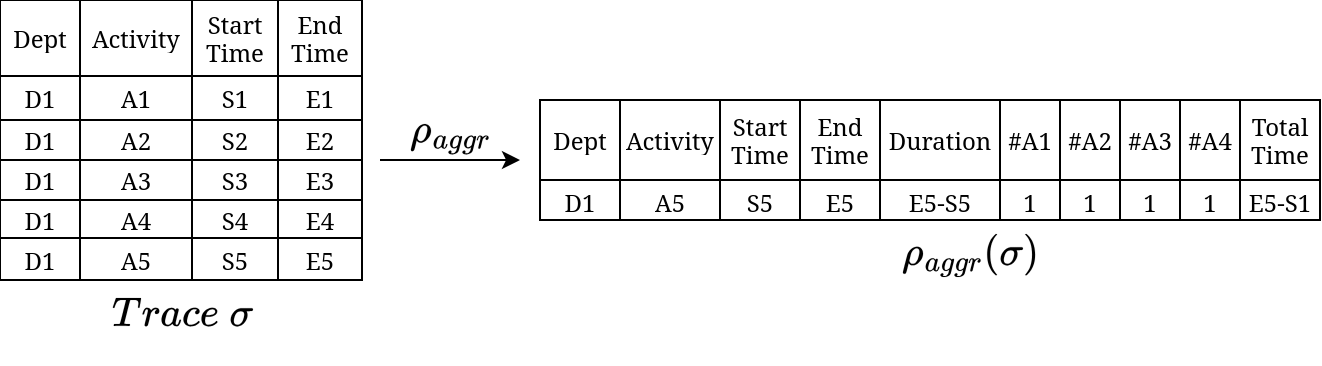
\includegraphics[width=\linewidth]{Figures/encoding.png}
    \caption{Example of an encoding function applied to a running trace used for predicting the KPI “total time”.}
    \Description{Output example of an Aggregated History encoding function, showing how past activities are encoded in new columns.}
    \label{fig:encoding}
\end{figure}

Figure~\ref{fig:encoding} depicts an example of a trace-to-instance encoding function $\rho_{aggr}$. The trace is flattened into a fixed-size feature vector in which each activity of the process is associated with a dedicated component recording the number of its past occurrences in the trace. This encoding enables the tracking of the absolute frequency of all past activities but does not preserve their sequential order, retaining information only about the most recent one. The trace-to-instance encoding function has been widely employed in PPM~\cite{10.1007/978-3-032-02936-2_15,bib:padella,DBLP:conf/bpm/PadellaMVLV24}.

% To formally define this encoding function we have to first define $\rho^{hist}_{\mathcal{A}}((\langle e_1, \ldots, e_n \rangle))$. Here, for each activity $a \in \mathcal{A}$, one dimension exists in $\rho^{hist}_{\mathcal{A}}(\sigma): \mathcal{E}^* \rightarrow (\NN)^{|A|}$ that takes on a value equal to the number of events $e_i\in\sigma$ such that $activity({e})=a$ for $i=1,\ldots,n$.
% The function $\rho_{aggr}$ is then defined as: $\rho_{aggr}(\langle e_1, \ldots, e_n \rangle)= global(\langle e_1,\ldots,e_n\rangle) \displaystyle\oplus activity(e_n) \displaystyle\oplus start(e_n) \displaystyle\oplus end(e_n) \displaystyle\oplus duration(e_n) \displaystyle\oplus local(e_n) \displaystyle\oplus \rho^{hist}_{\mathcal{A}}(\langle e_1, \ldots, e_n \rangle) \displaystyle\oplus end(e_n)-start(e_1)$. As reported in the Section~\ref{sec:intro}, this function has been widely adopted in the literature~\cite{DBLP:conf/bpm/RizziSFGKM19,DBLP:conf/bpm/BuligaVGLDFGR24,DBLP:journals/eaai/GalantiLMNMSM23}

% The second encoding in Figure~\ref{fig:encoding} is the \textit{Last-2 Encoding} method. It only records the last two activities, thereby preserving their order while partially disregarding the complete sequence of past activities. For this encoding we do not provide a formal definition, since it only serves as example and it will not be used in the pap

% Once the trace-to-instance encoding function is defined, it is possible to define the KPI function. 
% \begin{definition}[KPI function]\label{def:total_time_func}
%     Let $\sigma\in\ME^*$ be a trace defined as $\sigma = \left\langle e_1,\ldots,e_n \right\rangle$. Let $j$ be an integer such that $1 \leq j\leq n$, and let $\rho:\ML\rightarrow dom(\MT)$ a . The KPI function $\MT: dom(\MT)\times\NN\rightarrow\NN$ returns the value of $time(e_n)-time(e_1)$, after the occurrence of $j$ events.\footnote{The function's output consists of natural numbers since they can be expressed in UNIX notation.}
% \end{definition}

% However, the aim of this paper is to leverage the LLM to estimate the KPI of a running trace $\sigma'$. To this extent we introduce a general definition of it to establish the necessary conceptual framework:

% \begin{definition}[veriage Model]\label{def:llm}
% Let $\Sigma^*$ be the set of all finite strings over an alphabet $\Sigma$. A \textit{Large Language Model} (LLM) is here modeled as a function  $LLM:\Sigma^*\rightarrow\Sigma^*$ that, given an input $s \in \Sigma^*$, returns a string $LLM(s)$, which depends on the specific interpretation of the model.
% \end{definition}

% \noindent We are aware that this is a simplification of the actual reality; however, as this paper seeks to propose a method for enhancing prediction quality through the use of an LLM, we provide a broad, simplified mathematical definition of LLMs, solely for the purpose of providing a reference function. This prediction method has been adapted from a more formal framework introduced in~\cite{requeima2025llm}.



 %\todo{Alessandro e Paolo: Max qua abbiamo scritto il discorso di training/fine tuning che dicevamo a pranzo. Leggi e controlla. Massimiliano: in generale va bene, ed ho semplicemente indicato che lo facciamo "to keep the discussion simple".}
% We also loosely refer to training and testing logs to denote available and unseen data for evaluating our models. However, in this context, we do not properly train the LLMs, but rather pass the encoded training traces in its prompts, as described in more detail in the remaining part of this work.

\section{Approach For LLM-based Predictions}\label{sec:framework}

This study seeks to leverage the potential of LLMs to develop a framework for PPM, particularly in scenarios where only a small amount of example traces is accessible. Leveraging their embedded knowledge, LLMs can extract and use additional information beyond the event data by incorporating the semantics of events, such as activity names, that traditional models cannot. Figure~\ref{fig:pipeline} depicts the proposed approach. Given an event log of completed traces $\ML$ and a running trace $\sigma'$, a trace-to-instance encoding function $\rho$ is applied to transform them into a structured prompt. This prompt, composed of multiple components, is then used to enable the LLM to estimate the KPI function $\MK$. 

In the remainder of this Section, a new trace-to-instance encoding function $\rho_{seq}$ suitable for LLM is introduced in Section~\ref{subsec:framework_enc}, while Section~\ref{subsec:context} defines a context-based prompt suitable for employing an LLM for implementing the KPI function defined in Section~\ref{sec:prel}, while Section~\ref{subsec:explain} provides an example of LLM's output containing the predicted values and its reasoning to achieve it.

\begin{figure}[t!]
    \centering
     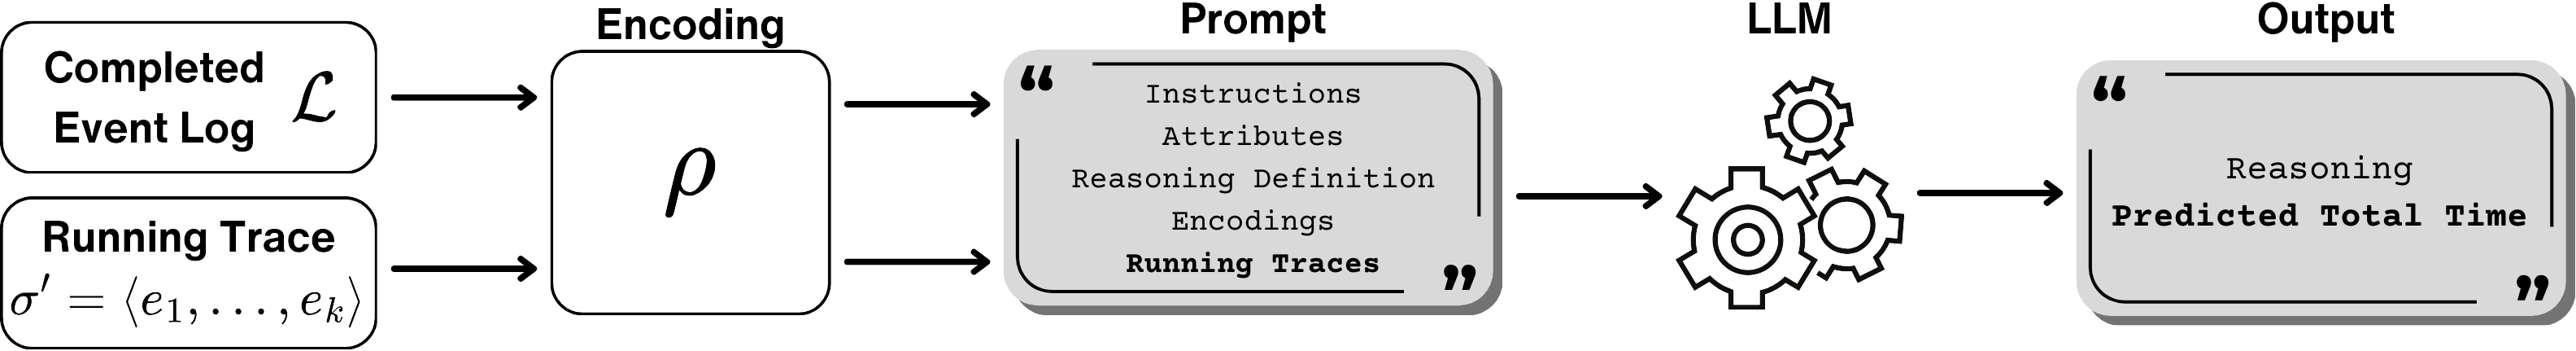
\includegraphics[width=1\linewidth]{Figures/pipeline.png}
    \caption{Pipeline outlining the proposed method using LLMs for PPM, in which the KPI is “total time”.}
    \Description{Placeholder}
    \label{fig:pipeline}
\end{figure}


\subsection{An Encoding Function for LLMs}\label{subsec:framework_enc}
% Exploiting an LLM for developing a PPM framework is a topic that has not yet been explored in process mining (cf.\ Section~\ref{sec:rw}). 
This section introduces a new LLM-suitable trace-to-instance encoding function $\rho_{seq}:\ME^*\rightarrow \Sigma^*$, where $\Sigma$ is the set of all the strings. % that is associated to an encoding that will be referred as \textbf{Sequential}. %This function takes as input

% an encoding function that generates a text-based representation of a log for LLMs, referred to as \textbf{Sequential}, and is associated with a trace-to-instance encoding function $\rho_{seq}$.


The input of the $\rho_{seq}$ function is a trace, while the output is a textual prompt enhanced to become suitable for an LLM. Specifically, in this case the generic input set of the KPI function $\MX$ is equal to $\Sigma^*$. In $\rho_{seq}$, each trace $\sigma=\langle e_1,\ldots,e_n \rangle$ is mapped into a string composed of three main elements:
\begin{itemize}
\item The names and values of the attributes trace attributes.
\item A sequence of tuples ${ \left(activity\left(e_i\right),duration\left(e_i\right)\right)\ for\ i=1,\ldots,n}$.
\item The actual value of $\MK(\sigma)$.
\end{itemize}
Formally:
\[
\scalebox{0.9}{$
    \begin{aligned}\rho_{seq}\left(\langle e_1,\ldots,e_n\rangle\right)=& \{(x, \pi_x(\sigma)) \mid x \in \mathcal{V}\} \displaystyle\oplus \left(activity\left(e_1\right),duration\left(e_1\right)\right)\displaystyle\oplus\ldots\displaystyle\oplus\notag \\&\left(activity\left(e_n\right),duration\left(e_n\right)\right)\displaystyle\oplus \left(k\right)
    \end{aligned}$}
\]
\footnote{Considering $\displaystyle\oplus$ as the concatenation of vectors e.g.\newline $[1,3,'request\_ created']\oplus[2,True]=[1,3,'request\_ created',2,True]$} 





\noindent
The sets of event-related attributes have been excluded, due to \textbf{technical} limitations and \textbf{methodological} considerations. From a technical perspective, an LLM can only process a certain number of characters and so it becomes necessary to reduce the size of the input to stay within this maximum quantity, namely the \textbf{Context Length}.\footnote{See \href{https://llm-stats.com/}{https://llm-stats.com/} for an overview of Context Lengths of the latest models.} Note that the Context Length of an LLM is not just a limitation per interaction (e.g., in a chatbot) but an inherent architectural constraint. From a methodological perspective, empirical evidence suggests that LLMs do not process input data uniformly: the contribution of individual elements to the model's output tends to decrease as the input sequence grows, with potential adverse effects on predictive performance~\cite{kuratov2024babilong,2024longcontext}. Therefore, we opted to omit event attributes. Conversely, trace attributes were retained since they incorporate domain knowledge and have generally proved to retain more predictive power than event ones (cf.\ Galanti et al. in~\cite{DBLP:journals/eaai/GalantiLMNMSM23}).

\begin{figure}
    \centering
    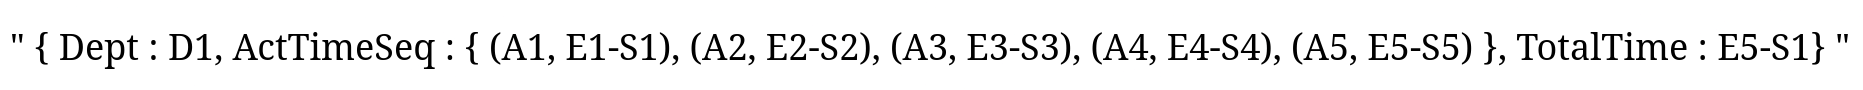
\includegraphics[width=\linewidth]{Figures/seqenc.png}
    \caption{Example of a usage of the Sequential encoding function $\rho_{aggr}$ applied to the same running trace and KPI employed in Figure~\ref{fig:encoding}.}
    \Description{Placeholder}
    \label{fig:seqenc}
\end{figure}
An example of application of the sequential trace-to-instance encoding function $\rho_{seq}$ is depicted in Figure~\ref{fig:seqenc}, where the example trace reported in Figure~\ref{fig:encoding} has been processed as a string. The result is a string-form object primarily composed of three keys: i) \textit{Dept}, associated with the value of the corresponding trace attribute; ii) \textit{ActTimeSeq}, associated with the list of tuples where each activity and its duration are recorded; and iii) \textit{TotalTime}, representing the total duration of the trace.

Since LLM prompts are arbitrary strings, alternative encodings are viable, such as a string representation of the aggregate encoding (cf.\ Figure~\ref{fig:encoding}), as the LLM can generate predictions independently of the specific encoding employed. This flexibility allows the framework to accommodate different encoding strategies, which have been explored in~\cite{10.1007/978-3-032-02929-4_16}. However, since the focus of this paper is on analyzing the reasoning mechanisms and semantic exploitation of LLMs rather than on comparing encoding strategies, we adopt the sequential encoding throughout, as it has been shown to yield the best predictive performance.

\subsection{Context-Based Prompting Technique for LLMs in Predictive Process Monitoring}\label{subsec:context}

This Section describes how traces encoded via the encoding function $\rho_{seq}$ are incorporated into an input prompt suitable for an LLM. In essence, we define a prompting technique that allows the model to make KPI predictions along with a corresponding reasoning procedure, starting from the encoded traces. %The prompting technique is divided into seven key parts, also reported in Listing~\ref{lst:train}:  
Listing~\ref{lst:train} illustrate an example of the prompt used to make prediction for a running trace. The prompt is composed by seven conceptual parts:

\begin{itemize}  
    \item \textbf{Initial instruction and Header:} The LLM is introduced to the task with the prompt:  
    \textit{“You are an expert in process mining and machine learning. Your task is to predict the KPI of process instances based on event logs of activities, where each process instance is a sequence of activities.”} This part varies based on the KPI employed, replacing the word “KPI” with the actual KPI of interest. In the example, the actual KPI is “total time” (Lines 1-2)

    \item \textbf{Attributes and Encoding description:} Contextual information specific to the process is provided, and the trace-to-instance encoding function is described ($\rho_{seq}$ in the example). (Lines 4-12)

    \item \textbf{Output and Reasoning format specification:} The expected structure for predicted values is defined, including placeholders for the step-by-step reasoning and the final answer. This enforces a consistent output format that facilitates both prediction extraction and subsequent analysis of the LLM's inferential process. (Lines 14-22 and 29-35)
    
    \item \textbf{Running Trace Format Specification:} The format for describing a running trace is specified to the model, distinguishing it from completed traces by means of a dedicated label (``Running'') that signals the process instance is still in progress. This allows the LLM to recognize that additional activities are expected before the case concludes. (Lines 24-27)
    
    \item \textbf{Domain-specific background information:} Additional details about the process from which the data has been extracted. (Lines 37-38)

    \item \textbf{Example Data Provision:} Encoded data is provided as example to the model. (Lines 39-45)

    \item \textbf{Running Trace Provision:} The running trace is provided in the same format as the examples, ending with a special place-holder activity “Running”, to signal the trace not be completed 24-27. (Lines 47-50)
\end{itemize}  


Although the proposed encoding is general and applicable to various use cases and KPI, certain information within these seven components must be specified by the process analyst and could be removed. 
\\
\lstset{
basicstyle=\fontsize{6.1}{8}\ttfamily,
    label={lst:train},
    numbers=left,
    caption={Prompting technique example for a loan application process (Bpi12), for the KPI of Total Time. Lines that have to be provided by the process analyst are marked in bold. In the example, only 2 training traces are provided due to space limitation.},
    captionpos=b,
    moredelim=**[is][\bfseries]{@}{@},
    float=t
} % Adjust scale as needed
\begin{lstlisting}
You are an expert in process mining and machine learning. Your task is to predict the 'total time' of 
process instances based on event logs, as each process instance is a sequence of activities.

A event log is a collection of traces, where each trace represents a process instance. 
Each trace is mapped as a sequence of activities and integers representing the minutes since the start
of the process.
The log is represented as a python list containing one dictionary for each trace. Included in it are:
@- the key "AMOUNT_REQ", representing the total amount of euros requested in the loan application.@
- the key "ActTimeSeq", which value is a list of [activity, cumulative elapsed minutes] 
- The key "total_time", which value is the total execution time in minutes from the start of the activity, 
that is the value to predict.

All interactions will be structured in the following way, with the appropriate values filled in.

[[ ## reasoning ## ]]
{your step-by-step reasoning}

[[ ## answer ## ]]
{your predicted total time as an integer}

[[ ## completed ## ]]

In adhering to this structure, your objective is to analyze the event log, and apply reasoning to predict 
the total time for a new case. This case belongs to a not-yet-completed process instance, represented by the 
label "Running" in "ActTimeSeq", indicating that more activities are expected before reaching the conclusion
of the process instance.

Ensure to articulate each step of your thought process in the reasoning field, detailing how you identify
relationships with past cases and leverage your intuition about the meaning of activities to arrive at the 
solution. The answer should be the final prediction of the total time for the given process instance.
Respond with the corresponding output fields, starting with the field [[ ## reasoning ## ]], 
then [[ ## answer ## ]], and then ending with the marker for [[ ## completed ## ]].

Your task is to learn from them and predict the 'total time' values for that traces.

@The process deals with a loan application process from a Dutch financial institution. It has been provided 
in the Business Process Intelligence (BPI) challenge in 2012. @
The following list shows some completed example cases with their total times:

     {"AMOUNT_REQ": 5000.0, "ActTimeSeq": [["W_Completeren aanvraag", 11],
     ["W_Nabellen offertes", 1464], ["W_Nabellen offertes", 7486]], "total_time": "7486"}
     {"AMOUNT_REQ": 15000.0, "ActTimeSeq": [["W_Completeren aanvraag", 13],
     ["W_Nabellen offertes", 14], ["W_Validate application", 4328], ["W_Validate application", 8792]], 
     "total_time": "8792"}
     ...
     ...
        
Now predict the total time for this new uncompleted case, considering that the case is still running:

    {"Application_1000386745": {"AMOUNT_REQ": 18000.0, 
    "ActTimeSeq": [["W_Completeren aanvraag", 2], ["W_Nabellen offertes", 8571], ["Running"]]}
\end{lstlisting} 

In Listing~\ref{lst:train} they have been highlighted in bold. They are specifically, (i) the domain-specific background information (Lines 36-37) and (ii) the description of the trace attributes (Lines 8-9), as they contain contextual details specific to the process under study.
Notably, these information pieces are optional and can be excluded if the process actor thinks that it is better to give more relevance to the provided example rather than the process description. The remaining sections of the prompt are designed to be generic and can be applied to any event log without modification.

This modularity ensures that the framework can be associated with any encoding function and eventually be customized with details about the single process, while minimizing the effort needed for customization when applying the LLM to different process datasets. 

\subsection{Example of Reasoning to Achieve Predictions}\label{subsec:explain}

The prompt proposed in Section~\ref{subsec:context} does not solely query the LLM to provide a KPI prediction, but instructs to report the reasoning procedure to achieve it. This implies that the LLM's output is not limited to return the predicted value: it also reports on the reasoning leveraged to make the prediction. This is in fact a form of explanation of the predictions, of which one example is given in Listing~\ref{lst:test}.
\\
\lstset{basicstyle=\fontsize{6.1}{8}\ttfamily, label={lst:test},
caption={LLM’s output and reasoning returned after the prompting technique example for a loan application proces},
captionpos=b, float=tb} % Adjust scale as needed
\begin{lstlisting}
[[ ## reasoning ## ]]
The new case is for an application with a 'AMOUNT_REQ' of 18000.  The process instance 
has executed activities 'W_Completeren aanvraag' and 'W_Nabellen offertes'.
The process is currently 'Running'. 
To predict the total time, we will look at historical cases with similar characteristics.

1. Filter for similar Application Type and Requested Amount:
   We focus on cases with 'AMOUNT_REQ' 
   in a range around 18000.0 (e.g., 10000.0 to 25000.0) to find comparable instances.

2. Identify relevant historical cases:
   From the provided log, we select the cases that match 'AMOUNT_REQ' within the range of 10000.0 to 25000.0. 
   We list their total times:
   10000.0: 9713, 10000.0: 18803, 11500.0: 4771, 12000.0: 18924, 12000.0: 8102,
   13000.0: 6645, 13000.0: 21550, 14000.0: 9713, 15000.0: 8049, 15000.0: 17011

3. Calculate the median total time:
   To get a robust estimate and reduce the impact of outliers, we calculate the median of these total times.
   Sorted total times: 4771, 5299, 5975, 5975, 6645, 6645, 7432, 8049, 8102, 9713, 9713, 
   12991, 13056, 17011, 17434, 18803, 18924, 19826, 21550, 71762.
   71762 is detected as an outlier and it will be removed from the analysis.
   Since there are 19 values, the median is the 10th value,
   which is 9713. Median = 9713.

4. Predict total time:
   We use the median total time of the similar historical cases as our prediction
   for the new running case.

[[ ## answer ## ]]
9713
[[ ## completed ## ]]
\end{lstlisting}

% Nonetheless, it is a valuable addition to this paper to report and comment on an instance of the prediction's reasoning given as output by the LLM. To do so, Listing~\ref{lst:test} reports the output returned by the LLM for Listing~\ref{lst:train}. 

The output is returned at the end (see line 30 of Listing~\ref{lst:test}). The reasoning of this example is as follows: the LLM focuses on the traces of the provided training log in which the request amount is in the range of 10000 to 25000 (see lines 7-9). This leads to 20 traces (see lines 15-16), for which the median value is computed (see lines 24-25), an outlier removed, and the median is used as predicted value (see explanations given at lines 28 and 29). 

This reasoning certainly provides a valid explanation of the motivation behind the reason this prediction is provided. However, this is only an example of the reasoning procedure by the LLM, and we observed that the reasoning can differ remarkably from one execution to another. whithin the same process.% & vary depending on the context and the number of training traces provided. % Effort is necessary to homogenize the output prompt, and to steer towards a solution that is more explainable for process stakeholders. The latter still requires a research investigation that involves users and multiple analysis. We aim to move towards this direction as future work. 

% The given reasoning explains the prediction, but it is only an example of the reasoning procedure that is performed by the LLM, which changes with context and data. To improve explainability for process stakeholders, a more consistent and standardize output is necessary. This requires in-depth research involving user studies and varied analytical methods, a direction we intend to explore as future work.



\section{Experimental Results}\label{sec:exps}

Section~\ref{sec:intro} introduced the three research questions we aim to address in this paper. To this exten, we design a set of experiments to assess the effectiveness of our approach in generating predictions in six real-life use cases, made of 3 different processes for which 2 different KPIs have been targeted. 
The remainder of this section is organized as follows: The use cases are presented in Section~\ref{subsec:use_cases} along with the analyzed KPIs of interest. Section~\ref{subsec:rq1} reports on the experimental design and the results plus a discussion, pertaining the first research question, while Section~\ref{subsec:rq2} and~\ref{subsec:rq3} do the same for the second and the third research question, respectively. 
%Section~\ref{subsec:traintest} reports how the logs have been divided into training and test sets for use in the experimental setup. Section~\ref{subsec:exp_pipeline} outlines the experimental pipeline employed to address the research questions posed in Section~\ref{sec:intro}, while Section~\ref{subsec:results} concludes with the results and their associated analysis.
% \todo[inline]{riformula}


\subsection*{Use Cases and Benchmarks}\label{subsec:use_cases}

Since this paper targets data-scarce environments, we simulate a scenario in which only 100 complete traces are available, evaluating the LLM against state-of-the-art benchmarks trained on the complete event log, across six different use cases composed by three distinct processes and two KPIs. To ensure the robustness of the evaluation, we sampled the 100 traces 20 times, capturing both the average quality of the models and the variability associated.

The evaluation leverages three different process, from which an event log has been extracted:

\begin{itemize}

\item \textbf{Bpi12}\enspace This loan application process has been used by the BPI challenge in 2012\footnote{https://doi.org/10.4121/uuid:3926db30-f712-4394-aebc-75976070e91f}, it contains 8,049 traces, 6 different activities and 1 trace attribute: \textit{Requested\_Amount}.

\item \textbf{Bac}\enspace A process referring to a Bank Institution that deals with the closures of bank accounts. It contains 32,429 completed traces, 15 different activities and 2 trace attributes: \textit{Closure\_Type}, and \textit{Closure\_Reason}.\footnote{https://github.com/IBM/processmining/tree/main/Datasets\_usecases}

\item \textbf{Hospital}\enspace This process has been provided by a Hospital emergency department. The log is made of 37,945 completed traces, contains 46 different activities and 3 trace attributes, that are \textit{Triage\_Color},\textit{Triage\_Access} and \textit{Patient\_Age}. Due to confidentiality, this event log cannot be published.

\end{itemize}

For each process, we consider two prediction tasks, corresponding to two different KPIs:

\begin{itemize}

\item \textbf{Total time} of an ongoing case, i.e., a regression task.

\item \textbf{Activity occurrence} for a selected target class, i.e. a classification task. 

\end{itemize}



\begin{table}[t]
    \centering
    \begin{tabular}{|c|c|c|c|}\hline
        \textbf{Process} & \textbf{$\ML^{comp}$ Size}  & \textbf{100/$\ML^{comp}$ Size}  & \textbf{Target Activity} \\\hline
         Bpi12&  6421 & 1.55\%&  W\_Nabellen incomplete dossiers\\\hline
         Bac & 25843 & 0.38\%& Service closure Request with BO responsibility\\\hline
         Hospital &  30394&  0.32\%& LABORATORIO\\ \hline
    \end{tabular}
    \caption{Overview of the analyzed use cases, including the number of available training traces, the relative proportion represented by 100 traces, and the target activity selected for the KPI activity occurrence.}
    \label{tab:use_cases}
\end{table}



Table~\ref{tab:use_cases} summarizes the processes employed with their related statistics, also reporting the ratio that 100 traces represent relative to the total size of $\ML^{comp}$. The first column reports on the process, whereas the second and third columns indicate the number of traces in $\ML^{comp}$ and the percentage value that 100 traces represent out of the total number, respectively. Finally, the last column identifies the target activity for the KPI prediction task of activity occurrence. These target activities were selected because their execution typically leads to both higher time and cost demands. In the Bpi12 use case, the target activity is “\texttt{W\_Nabellen incomplete dossiers}”, which translates to “Follow up on incomplete files.” This activity occurs when an error in the loan application process requires rework by both sides of the bank and the customer. A similar pattern is observed for the activities “\texttt{Service Closure with BO Responsibility}” and “\texttt{LABORATORIO}”, which signal the need for further laboratory analysis, implying implying additional Hospital processing and resource usage.

\noindent
For the purpose of setting a benchmark for prediction, we employed two different state-of-the-art techniques for the different KPIs of interest:

\begin{itemize}

\item For total time we employed PGTNet architecture from~\cite{DBLP:conf/caise/ElyasiAS24} that has proven to outperform every PPM framework. However, we also report results in terms of CatBoost regression since in~\cite{galanti2020explainable} it has proven to obtain competitive performance with a very limited computational time required, constituting a valid alternative to PGTNet.

\item For the activity occurrence, we employed CatBoost Classifier from~\cite{CatBoost}, a state-of-the-art model predictor based on machine learning with decision trees, which has been shown to surpass existing prediction frameworks~\cite{galanti2020explainable}.

\end{itemize}

Since the PGTNet architecture has been designed exclusively for regression tasks, it is not applicable to activity occurrence prediction tasks and is therefore omitted from the corresponding benchmark comparison.

The whole approach has been implemented in Python and the code is publicly available.\footnote{\url{https://github.com/Pado123/gui_xrecs_presc_analytics}}. The KPI function development has been carried on using \textbf{Gemini 2.5 Flash Thinking}: a state-of-the-art LLM developed by Google DeepMind~\footnote{\url{https://gemini.google.com/app}}, but any choice of LLM is valid. The model is built on a multimodal architecture designed for advanced natural language understanding and generation. As the development of LLMs progresses, we anticipate that the performance of upcoming models using our method may see fast improvements, that can be tracked in~\cite{llms_leaderboard}

\subsection{RQ1: Prediction Quality Comparison}\label{subsec:rq1}
This research question extends the experimental part of~\cite{10.1007/978-3-032-02929-4_16} and addresses RQ1: \textit{When trained on event logs with a limited number of traces, do LLMs achieve superior prediction quality on a wide range of metrics, compared to the models available in literature?}

\subsubsection{Experimental Setup}

According to standard supervised learning practices, we divided the event log $\ML$ into training and test, $\ML^{comp}$ and $\ML^{run}$, respectively. To extract the training log, we compute the earliest time $t_{split}$ such that $80\%$ of the identifiers related to traces of $\ML$ are completed. This allows us to define $\ML^{comp}$ as the set of traces of $\ML$ completed at time $t_{split}$, and consequently, define $\ML^{run}$ as $\ML \setminus \ML^{comp}$. The traces of the test log $\ML^{run}$ are truncated to a set $\ML^{trunc}$, namely the set of prefixes, that is obtained from $\ML^{run}$ by removing every event with a timestamp larger than $t_{split}$: $\ML^{trunc}$ only contains the events that occurred before time $t_{split}$. This procedure tries to mimic the reality at time $t_{split}$ and it is in line with the principles introduced in~\cite{DBLP:conf/bpm/WeytjensW21a}. The system is trained on $\ML_{comp}$, the predictions are produced for $\ML_{trunc}$ and tested using its completed form, $\ML_{run}$. Furthermore, to ensure the benchmarks' results were valid and significant, we randomly picked 10\% of traces and used them as a validation set $\ML_{valid}$ to apply a Cross-Validation approach needed for internally tuning the hyperparameters of the benchmarks. This technique is a widespread technique in PPM works~\cite{DBLP:conf/coopis/LeoniP24,10.1007/s10618-025-01117-3,PEEPERKORN2024102330}.

It is also worthwhile pointing out that in this paper we use the term \textit{training} to refer to both LLMs and machine-and-deep learning benchmark models, to keep the discussion simple. However, \textbf{we acknowledge that LLMs are already pre-trained: traces are provided to the LLMs as background, and are not formally used to train its internal parameters.}

We measured the accuracy of the LLM when trained on 100 traces sampled from $\ML^{comp}$, a substantially limited amount if compared to the benchmarks, which are trained on the complete training set (cf.\ Table~\ref{tab:use_cases}). 

To assess the performance of each prediction model, two metrics are employed, depending on the KPI of interest:

\begin{itemize}
\item \textbf{Mean Absolute Error (MAE)} \enspace
For total time prediction, the Mean Absolute Error is used:
\[
    MAE = \frac{1}{n}\mysum |k_i - \hat{k}_i|
\]

where $k_i$ is the actual total time, reported in minutes, $\hat{k}_i$ is the predicted value, and $n$ is the number of running traces. Lower MAE values indicate better predictive performance.

\item \textbf{F1-Score} \enspace
For activity occurrence prediction, the F1-Score is used:

$$\text{F1-Score} = 2 \cdot \frac{\text{Precision} \cdot \text{Recall}}{\text{Precision} + \text{Recall}}$$

where $\text{Precision} = \frac{TP}{TP + FP}$ and $\text{Recall} = \frac{TP}{TP + FN}$, with $TP$, $FP$, and $FN$ denoting true positives, false positives, and false negatives.

\end{itemize}

% Since these 100 traces have been randomly sampled for each run, we repeated the experiments 20 times in order to assess statistical validity, which motivates why the resulting values of MAE/F1-Score are reported associated with the corresponding standard deviation, indicated after the symbol $\pm$ in the remainder of this paper. When the benchmarks are trained on the whole $\ML^{comp}$, the standard deviation is not reported since there is no sampling.

We acknowledge that in our prior work we examined model performance when trained on 2 and 10 traces. However, the scope of this extension is orthogonal, as it focuses on analyzing the behavior and responses of the LLM in terms of their quality and not in terms of pure performance, while still analyzing use cases where the training set comprises at most 1.45\% of the total dataset. Furthermore, due to the context length limitation (cf.\ Section~\ref{sec:framework}) we could not test the LLM in the context in which all the event log $\ML^{comp}$ provided as training.

\subsubsection{Results}

\begin{table}[t]
\centering
\caption{MAE (minutes) results}
\begin{tabular}{|l|l|l|l|}
\hline
\textbf{Use Case} & \textbf{Model} & \textbf{all\_df} & \textbf{100 Traces}  \\
\hline
\multirow{3}{*}{Bpi12}
& CatBoost Regressor  & $6846 $ & $9394 \pm\ 1275$ \\
& PGTNet  & $3888 $ & $8856 \pm\ 576$ \\
& LLM &- & \textbf{6508} $\pm\ 235$ \\
\hline
\multirow{3}{*}{Bac}
& CatBoost Regressor  & $2647 $ & $6393 \pm 365$ \\
& PGTNet  & $1245 $ & $4753 \pm 472 $ \\
& LLM  &- & \textbf{2265} $\pm\ 1072$ \\
\hline
\multirow{3}{*}{Hospital}
& CatBoost Regressor &253 & $259 \pm 52$ \\
& PGTNet  &97 & $132 \pm 32$ \\
& LLM  &- & \textbf{115} $ \pm\ 34$ \\
\hline
\end{tabular}
\label{tab:mae_results}
\end{table}

\begin{table}[t]
\centering
\caption{F1-Score results}
\begin{tabular}{|l|l|l|l|}
\hline
\textbf{Use Case} & \textbf{Model}  & \textbf{all\_df} & \textbf{100} $\pm$ \\
\hline
\multirow{2}{*}{Bpi12}& CatBoost Classifier & 0.80& 0.72 $\pm$ 0.07\\
& LLM & - & \textbf{0.77} $\pm$ 0.06\\
\hline
\multirow{2}{*}{Bac}& CatBoost Classifier & 0.95& 0.78 $\pm$ 0.08\\
& LLM  &-& \textbf{0.98} $\pm$ 0.04\\
\hline
\multirow{2}{*}{Hospital}& CatBoost Classifier &0.90& \textbf{0.90} $\pm$ 0.01\\
& LLM  & - & \textbf{0.90} $\pm$ 0.08\\
\hline
\end{tabular}
\label{tab:f1-score_results}
\end{table}


Table~\ref{tab:mae_results} reports the MAE in minutes for total time prediction across the Bpi12, Bac, and Hospital use cases, comparing the LLM against the CatBoost Regressor and PGTNet benchmarks introduced in Section~\ref{subsec:use_cases}. The first column reports on the process employed, the second the model, while the third and fourth columns report the MAE when the models are trained on the full event log (\texttt{all\_df}) or on only 100 traces (\texttt{100 Traces}), respectively.

For the Bpi12 use case, the LLM achieves a competitive MAE of $6508 \pm 235$, comparable to the performance of CatBoost trained on the entire event log ($6846$) and substantially better than the same model trained on 100 traces ($9394 \pm 1275$). Compared to PGTNet, the LLM falls short of the full-log configuration ($3888$) but clearly outperforms the small-scale one ($8856 \pm 576$). 

A consistent pattern emerges for the Bac use case, where the LLM ($2265 \pm 1072$) consistently outperforms both CatBoost Regressor ($6393 \pm 365$) and PGTNet ($4753 \pm 472$) in the small-scale setting. When the benchmarks are trained on the full training set, the LLM matches CatBoost and is only surpassed by PGTNet, which is the strongest dedicated regression model in the comparison.

For the Hospital use case, the LLM ($115 \pm 34$) outperforms both CatBoost ($259 \pm 52$) and PGTNet ($132 \pm 32$) trained on 100 traces, although the standard-deviation intervals partially overlap with PGTNet. Notably, the LLM also surpasses both benchmarks even when they are trained on the entire event log ($253$ and $97$, respectively), suggesting that the richer set of trace attributes available in this domain (patient age, arrival modality, and triage color) is effectively exploited by the LLM through its embodied knowledge.

Table~\ref{tab:f1-score_results} reports the F1-Score for the activity occurrence prediction task, with CatBoost Classifier as the benchmark. As in Table~\ref{tab:mae_results}, the benchmark results are reported under both training configurations.

When restricted to 100 training traces, the LLM outperforms CatBoost in two out of three use cases (Bpi12: $0.77 \pm 0.06$ vs $0.72 \pm 0.07$; Bac: $0.98 \pm 0.04$ vs $0.78 \pm 0.08$) and matches it in the third (Hospital: both $0.90$). When compared against CatBoost trained on the entire event log, the LLM still surpasses it on Bac ($0.98$ vs $0.95$), matches it on Hospital ($0.90$ vs $0.90$), and trails it on Bpi12 by a narrow margin of $0.03$.

Taken together, these results indicate that the LLM consistently delivers competitive or superior predictive performance in data-scarce settings, while remaining largely on par with state-of-the-art benchmarks even when the latter are trained on the complete event log. This is particularly noteworthy considering that the LLM operates without any task-specific training, relying solely on the 100 example traces provided within the prompt.


\subsection{RQ2: String Anonymization of the Input Prompts}\label{subsec:rq2}
The second step of the experimental pipeline addresses RQ2: \textit{Do LLMs leverage their embodied prior knowledge of the process domains to improve predictions?}


\subsubsection{Experimental Setup}
The goal of this section is to replicate the experiments after replacing the semantic content from attribute names and values, while preserving the underlying data correlations and value distributions. To this end, each string-typed attribute name and value is replaced by a fixed, unique 4-character random identifier.

To isolate semantic understanding from distributional patterns, we anonymize all context-sensitive strings that could enable the LLM to exploit domain knowledge. Traditional machine-and-deep learning methods remain unaffected by string anonymization since they operate on numerical encodings, conversely LLMs with embodied knowledge may leverage activity semantics. For instance, the activity name “LABORATORIO” implies laboratory analysis, but also and attribute names such as, “Triage\_Color” suggests emergency care. This leads to the fact that we have to anonymize not only the values of the categorical attributes and activities, but also the name of those attributes since they provide information about the process context.

We define the context-sensitive set $\MH$ as:
\begin{equation}
\MH = \MA \cup \left( \bigcup_{i=1}^n \{v \in \MV_i \mid \text{type}(\MV_i)=\text{global}\} \right) \cup \left( \bigcup_{i=1}^n \{\text{name}(\MV_i) \mid \text{type}(\MV_i)=\text{global}\} \right)
\end{equation}

Based on it, a deterministic hash function $Hash: \MH \to \Sigma^4$ maps each $s \in \MH$ to a unique 4-character identifier ($c_1c_2c_3c_4$, $c_i \in \Sigma$), preserving correlations while eliminating semantics. 

In this experimental pipeline's phase, after the prompt generation as outlined in Section~\ref{sec:framework}, every $s \in \MH$ is replaced by $Hash(s)$. Then, the prediction quality in terms of MAE or F1-Score is compared between hashed and non-hashed prompts to quantify the semantic dependency of the LLM. Significant performance degradation under hashed prompts indicates that the LLM is relying on its embodied knowledge. 

\begin{figure}[t!]
    \centering
    \includegraphics[width=.99\linewidth]{Figures/hashed_trace.pdf}
    \caption{Example of the Hashing procedure applied to the trace in the Figure~\ref{fig:seqenc}.}
    \label{fig:enchashed}
\end{figure}

An example of how the traces after being encoded through the function $\rho_{seq}$ are hashed is depicted in Figure~\ref{fig:enchashed}, in this case, the context-sensitive set $\MH$ is $\MH = \{Dept,\ D1, A1, A4\}$ since the variable name “Dept” can be associated to some organization-related context, as do its value and the activity names, while the activity durations $E1-S1$ are only numbers that do not need to be hashed. This procedure also removes the context-related information that has been added to the prompt (cf.\ bold sentences in Listing~\ref{lst:train}). We remind that this is only the hashing procedure for a given trace, a full example of hashed input prompt and its associated output from the LLM are reported in the Appendix, at Listings~\ref{lst:hashed_ao} and~\ref{lst:hashed_ao_answ}.

Furthermore, we aim to assess the statistical significance of the accuracy in the predictions when attribute names and values are or are not replaced with their anonymized representation. To this extent we applied the Nemenyi post-hoc test across repeated experiments:

The Nemenyi test, from Nemenyi~\cite{nemenyi1963}, is a global statistical test (such as the Friedman test) that serves to investigate if it is possible to reject the null hypothesis that the reaction of the same group of individuals subject to 2 different treatments is the same. The test makes pair-wise tests of performance and we apply it on every running trace under the following hypothesis: 

\begin{itemize}

    \item Null hypothesis ($H_0$): No significant difference exists between prediction performance (MAE/F1-Score) of hashed and non-hashed prompts across use cases.

    \item Alternative hypothesis ($H_1$): Significant performance difference exists, with non-hashed prompts expected to outperform due to semantic exploitation.
    
\end{itemize}



% \paragraph{(1) LLM-feasible encoding introduction.}

% To enable LLM-based predictions in predictive process monitoring, a dedicated trace-to-instance encoding function $\rho$ is designed to transform event log traces into structured textual prompts that preserve the sequential order of activities, trace attributes, and event durations while remaining concise to respect the LLM's context length constraints.







\subsubsection{Results}

\begin{table}[t!]
\centering
\caption{Comparison between LLM and LLM hashed prompts with Nemenyi Post-Hoc Test Results}
\begin{tabular}{l l c c c c c}
\hline
\textbf{KPI} & \textbf{Use Case} & \textbf{LLM} & \textbf{LLM hashed} & \textbf{Difference} & \textbf{P-value} & \textbf{Significance} \\
\hline
\multirow{3}{*}{Total Time (MAE)}
& Bpi12 & $6508 \pm 235$ & $9246 \pm 873$ & 42.06\% & 0.002 & ** \\
& Bac & $2265 \pm 1072$ & $3880 \pm 3254$ & 71.25\% & $<$0.001 & *** \\
& Hospital & $115 \pm 34$ & $2077 \pm 232$ & 1702\% & 0.002 & ** \\
\hline
\multirow{3}{*}{Activity Occurrence (F1)}
& Bpi12 & $0.77 \pm 0.06$ & $0.74 \pm 0.06$ & 0.03 & 0.018 & * \\
& Bac & $0.98 \pm 0.04$ & $0.96 \pm 0.04$ & 0.02 & 0.040 & * \\
& Hospital & $0.90 \pm 0.08$ & $0.84 \pm 0.06$ & 0.06 & $<$0.001 & *** \\
\hline
\end{tabular}
\label{tab:nemenyi_summary}
\end{table}


Table~\ref{tab:nemenyi_summary} outlines the results on the Nemenyi tests to address RQ2. The first and second columns respectively report the KPI and the corresponding use case, while the third column presents the difference between the hashed and non-hashed treatments. Because lower values of MAE are preferable, whereas higher values of the F1-Score are desirable, the direction of the difference in the third column varies across metrics. Specifically, for the KPI total time, the difference is computed as hashed $-$ non-hashed, whereas for the F1-Score, it is computed as non-hashed $-$ hashed. The fourth column reports the p-value of the Nemenyi test, along with the significance reported in the third column, where * implies $p<0.05$, ** implies $p<0.01$ and *** implies $p<0.001$, according with the standards in statistical inference.

All comparisons reject the null hypothesis of no difference between hashed and non-hashed prompts, confirming the LLM's reliance on semantic embodied knowledge. For total time prediction, effect sizes are substantial, also reaching a 1702\% difference in Hospital use case. These findings, aligned with MAE/F1 trends in Tables~\ref{tab:mae_hash} and \ref{tab:f1-score_results}, demonstrate that LLMs exploit event semantics. 



\subsection{RQ3: $\beta$-learners Derivation and Implementation}\label{subsec:rq3}

The third step of our experimental pipeline addresses RQ3: \textit{Do LLMs use an ensemble of different prediction models? If so, how would this take place?}

\subsubsection{Experimental Setup: Derivation and Re-implementation of LLM's $\beta$-learners}

To investigate this question, we manually analyzed 50 LLM output prompts, yielding a total of 150 reasoning traces per KPI. The output prompts contain reasoning explanations per use case and KPI. Following the visualization methodology proposed in \cite{zhou2025landscapethoughtsvisualizingreasoning}, we systematically cataloged recurring prediction patterns extracted from these textual explanations. Specifically, the aim of this part is to identify how the LLM reasoning changes the modality to provide its predictions, based on the reasoning procedure that it reported and that was requested in the prompt reported in the Listing~\ref{lst:train}.

These recurring prediction patterns were abstracted into families: the so-called $\beta$-learners. In this context, a $\beta$-learner constitutes a mathematically defined and reproducible model that explicitly performs the reasoning strategies that the LLM documented, and may be employed as KPI function (cf.\ Section~\ref{sec:prel}). %The full catalog of $\beta$-learner families, their derivation rationale, and Python implementations are detailed in Appendix~\ref{app:beta-learners}.

This analysis revealed that the groups of $\beta$-learners were consistent across the same KPI, which led us to classify them solely by KPI rather than by use case and KPI. Later, every derived $\beta$-learner is applied to the same test set $\ML^{trunc}$ introduced in~\ref{subsec:traintest} to produce KPI predictions. Then, the predictions from every $\beta$-learner have been evaluated in terms of MAE/F1-Score and the results compared with the LLM's. 

Furthermore, the statistical significance of performance differences is assessed via Wilcoxon signed-rank test ($\alpha = 0.05$) with the following hypotheses for each $\beta$-learner vs. LLM comparison with the following hypotheses:

\begin{itemize}
\item \textbf{Null hypothesis ($H_0$)}: No significant difference exists between prediction performance (MAE/F1-Score) of the current $\beta$-learner and the one obtained by the LLM.

\item \textbf{Alternative hypothesis ($H_1$)}: A significant difference exists between prediction performance (MAE/F1-Score) of the current $\beta$-learner and the one obtained by the LLM.
\end{itemize}

Then, to assess whether the LLM’s predictions merely replicate the strategies of individual $\beta$-learners or if they demonstrate more advanced inferential behavior, we compared the prediction performance by testing each $\beta$-learner only on the running trace in which the LLM has been classified using that $\beta$-learner. Specifically, for each $\beta$-learner, we isolated the subset of the 50 analyzed traces where the LLM was classified as following that learner’s approach and then compared the LLM’s prediction accuracy to that of the corresponding $\beta$-learner on the same subset, reporting the difference in terms of MAE or F1-Score. 

Since we acknowledge that merely reading and classifying the LLM's reasoning may not be enough to discover every possible $\beta$-learner. With the aim to assess the completeness of the $\beta$-learners definition process, we employ \emph{Good-Turing frequency estimation}. This statistical technique, originally developed for natural language processing and machine translation, provides a principled framework for estimating the probability of a new unseen event based on the frequency distribution of observed ones~\cite{good1953population}.

The Good-Turing formula estimates the adjusted probability of an item that has been observed $r$ times as:
\begin{equation}
P^*(r) = \frac{(r+1) \cdot N_{r+1}}{N_r \cdot N}
\label{eq:good_turing}
\end{equation}

where:
\begin{itemize}
\item $N_r$ denotes the number of $\beta$-learner patterns that have been observed exactly $r$ times in the training set of 50 derived patterns,
\item $N_{r+1}$ denotes the number of patterns observed exactly $(r+1)$ times,
\item $N$ is the total number of pattern occurrences,
\item $P^*(r)$ is the smoothed probability estimate.
\end{itemize}

The probability of observing a \emph{new} (never before seen) $\beta$-learner is estimated as:

\begin{equation}
P_0 = \frac{N_1}{N}
\label{eq:good_turing_unseen}
\end{equation}

where $N_1$ is the number of $\beta$-learner patterns observed exactly once in the training set.

This approach allows us to compute the expected number of novel $\beta$-learners $E[\text{novel}]$ that would be encountered when applying the method to $m$ new prediction instances (where $m \in \{1, 10, 100\}$):

\begin{equation}
E[\text{novel}] = m \cdot P_0 = m \cdot \frac{N_1}{N}
\label{eq:expected_novel}
\end{equation}

\subsubsection{Results}


For the prediction of the KPI total time, the extracted $\beta$-learners are:

\begin{itemize}
\item \textbf{knn act + mean/median/mode}: where the LLM based its prediction considering the $ActTimeSeq$ part of the Sequential encoding (cf.\ Figure~\ref{fig:seqenc}), this has been re-implemented using a $k$-nearest neighbors algorithm on activity-based representations with different aggregation functions, that at the end as predictor may use the mean, the median or the mode as predictor.

\item \textbf{knn att + mean/median/mode}: where the LLM based its prediction considering the attribute-related part of the Sequential encoding (cf.\ Figure~\ref{fig:seqenc}), this has been re-implemented using a $k$-nearest neighbors algorithm on attribute representations with different aggregation functions, that at the end as predictor may use the mean, the median or the mode as predictor.

\item \textbf{time seq + mean/median/mode}: where the LLM based its prediction considering the $ActTimeSeq$ part of the Sequential encoding (cf.\ Figure~\ref{fig:seqenc}), this has been re-implemented using a $k$-nearest neighbors algorithm on activity-duration representations with different aggregation functions, that at the end as predictor may use the mean, the median or the mode as predictor.

\item \textbf{path pred + mean/median/mode}: where the LLM based its prediction trying to infer which may be the probable next activity path, and their associated duration. The LLM considers the available training traces and merges them to predict the remaining time. this has been re-implemented using a $k$-nearest neighbors algorithm that analyzes the possible next activities with their associated durations, then leverages different aggregation functions, that at the end as predictor may use the mean, the median or the mode as predictor.

\end{itemize}

For prediction of the KPI activity occurrence, different $\beta$-learners have been identified:

\begin{itemize}
\item \textbf{Activity-Based}: This learner focuses on the sequence of executed activities, identifying similarities between traces based on their activity order and structure. This has been re-implemented with a tree-based predictor that provides the likelihood of the given activity’s occurrence by referencing similar past activity patterns.

\item \textbf{State-Based}: This learner evaluates the latest event in the trace, considering its associated duration and activity and identifying similar trace states. This has been re-implemented with a tree-based predictor that provides the likelihood of the given activity’s occurrence by referencing similar past activity patterns.

\item \textbf{Att-Based}: This learner evaluates the attribute values in the trace, considering its associated duration and identifying similar trace states. This has been re-implemented with a tree-based predictor that provides the likelihood of the given activity’s occurrence by referencing similar past activity patterns.

\item \textbf{Positive Evidence}: This learner simply verifies whether the target activity has already occurred within the current trace, using this as direct evidence to inform prediction. When the activity has not already occurred, it randomly guesses the output.

\end{itemize}

% The details on how the single $\beta$-learners have been implemented are reported in the code url.

\begin{table}[t!]
\centering
\resizebox{.9\textwidth}{!}{\begin{tabular}{|l|l|l|l|c|c|c|c|}
\hline
\textbf{Use Case} & \textbf{Model} & \textbf{all\_df} & \textbf{\textbf{100} $\pm$} & \textbf{\#best50 no} & \textbf{Significance}  & \textbf{Occurrence}  & $\Delta$\textbf{LLM when occurring}\\
\hline
\multirow{13}{*}{Bpi12}
& LLM & -  & \textbf{6508} $\pm 235$ & 39 &-  &- &-\\
& knn act mean  & 8356 & $8651 \pm 393$ & 2 & ***  &5 & 6\%\\
& knn act median  & 8082 & $8780 \pm 524$ & 2 & ***  &5 & 8\%\\
& knn act mode  & 13463 & $13200 \pm 1002$ & 0 & ***  &6 & 9\% \\
& knn att mean  & 13261 & $8974 \pm 245$ & 1 & ***  &4 & 75\%\\
& knn att median  & 14253 & $8957 \pm 453$ & 0 & ***  &2 & 51\%\\
& knn att mode  & 14591 & $16077 \pm 1690$ & 0 & ***  &4 & 24\%\\
& time seq mean  & 8764 & $9127 \pm 537$ & 1 & ***  &3 & 26\%\\
& time seq median  & 8016 & $8614 \pm 772$ & 4 & ***  &6 & 7\%\\
& time seq mode  & 12433 & $12710 \pm 1636$ & 0 & ***  &5 & 9\%\\
& path pred mean  & 15023 & $15060 \pm 3087$ & 0 & ***  &4 & 23\%\\
& path pred median  & 12349 & $13468 \pm 2819$ & 1 & ***  &4 & 23\%\\
& path pred mode  & 8546 & $15998 \pm 4578$ & 0 & ***  &6 & 11\%\\
\hline

\multirow{13}{*}{Bac}

& LLM & -  & \textbf{2265} $\pm 874$ & 36 &-  &- &-\\
& knn act mean  & 3994 & $6788 \pm 3972$ & 1 & *** &4 & 24\%\\
& knn act median  & 3563 & $3095 \pm 437$ & 4 & **  &9 & 10\%\\
& knn act mode  & 3372 & $5503 \pm 3434$ & 0 & **  &6 & 22\%\\
& knn att mean  & 21296 & $8094 \pm 2874$ & 0 & ***  &3 & 41\%\\
& knn att median  & 5401 & $4678 \pm 1969$ & 1 & **  &3 & 22\%\\
& knn att mode  & 5379 & $14964 \pm 879$ & 1 & ***  &3 & 11\%\\
& time seq mean  & 6917 & $9224 \pm 3820$ & 0 & ***  &2 & 8\%\\
& time seq median  & 6966 & $3916 \pm 531$ & 1 & ***  &5 & 12\%\\
& time seq mode  & 8702 & $9534 \pm 4135$ & 0 & ***  &1 & 22\%\\
& path pred mean  & 54692 & $6843 \pm 3820$ & 0 & ***  &6 & 61\% \\
& path pred median  & 3569 & $3249 \pm 445$ & 4 & ***  &9 & 8\%\\
& path pred mode  & 190092 & $5927 \pm 2699$ & 0 & ***  &4 & 6\%\\
\hline

\multirow{13}{*}{Hospital}
& LLM & -  & \textbf{115} $\pm 60$ & 45 &-  &- &-\\
& knn act mean  & 167 & $442 \pm 379$ & 0 & **  &4 & 24\%\\
& knn act median  & 388 & $175 \pm 15$ & 1 & **  &7 & 11\%\\
& knn act mode  & 458 & $503 \pm 653$ & 0 & ***  &2 & 12\%\\
& knn att mean  & 617 & $566 \pm 437$ & 0 & ***  &3 & 12\%\\
& knn att median  & 189 & $183 \pm 27$ & 1 & ***  &5 & 80\%\\
& knn att mode  & 1479 & $626 \pm 546$ & 0 & ***  &7 & 68\%\\
& time seq mean  & 661 & $670 \pm 805$ & 0 & ***  &4 & 11 \%\\
& time seq median  & 684 & $287 \pm 677$ & 0 & ***  &2 & 61\%\\
& time seq mode  & 643 & $708 \pm 771$ & 1 & ***  &4 & 34\%\\
& path pred mean  & 383 & $382 \pm 320$ & 0 & ***  &4 & 32\%\\
& path pred median  & 159 & $174 \pm 15$ & 2 & **  &4 & 14\%\\
& path pred mode  & 282 & $473 \pm 618$ & 0 & ***  &7 & 31\%\\
\hline
\end{tabular}}
\caption{Complete MAE results across all use cases and models, also paired with the possible outcome of $\beta$-learners.}
\label{tab:mae_results}
\end{table}

Tables \ref{tab:mae_results} present the MAE results describing the $\beta$-learners’ predictive performance compared to the LLM. The table systematically compares the re-implementations of the LLM’s reasoning patterns, i.e., the $\beta$-learners such as knn-act/att-mean/mode (nearest neighbors on activity/attribute features), time-seq-mean (temporal sequence aggregation), and path-pred-mean/mode (predicted future path estimation), across all three use cases under both the full $\ML^{comp}$ and when trained on 100 traces. The first use case and the model employed are reported in the first and second column respectively, while the third and the fourth column report on the MAE when the LLM or the $\beta$-learner has been trained on the whole training log or 100 samples respectively. The fifth column with header \textit{\#best50 no} reports the number of times the predictor achieves the lowest MAE for each running traces, i.e. how many times the corresponding model was the best one. The six column headed with \textit{Significance}, reports the significance of the Wilcoxon test with the hypothesis reported in Section~\ref{subsubsec:beta_learners} and the seventh column \textit{Occurrence} reports the number of times the LLM's answer has been classified as the corresponding $\beta$-learner. Finally, the eight column headed \textit{$\Delta$ LLM when occurring} reports the percentage difference in terms of MAE between the results obtained by the $\beta$-learner and the LLM, only for the running traces in which the LLM has been classified employing that corresponding $\beta$-learner. 

From them, it is possible to infer how the LLM outperforms not only the derived $\beta$-learner in the scenario in which they are trained on 100 samples, but also when the learners have been trained on the whole event log. This is further confirmed by the column \textit{\#best50 no}, which reports that the LLM obtains the lowest MAE in 39, 36 and 45 cases out of 50, respectively. Also, the column \textit{$\Delta$ LLM when occurring} proves that the LLM does not simply replicate the contribution of the $\beta$-learners, but does more articulate and complex pattern reasoning. An example of this can be viewed in the Listing~\ref{lst:test}, at the last point of the reported reasoning procedure. In fact, the LLM not only aggregates results in a range of values of “AMOUNT REQ” that are similar to the ones of the running trace (i.e. employing the $\beta$-learner of \textit{knn att + median}), but also removes a value that is considered as an outlier since its value is considerably higher than the rest of the values.


Tables \ref{tab:f1_beta} present the F1-Score results describing the $\beta$-learners’ predictive performance compared to the LLM. The table systematically compares the re-implementations of the LLM’s reasoning patterns, i.e., the $\beta$-learners such as Activity-Based (sequence of activities prediction), across all three use cases under both the full $\ML^{comp}$ and when trained on 100 traces. The first use case and the model employed are reported in the first and second column respectively, while the third and the fourth columns report on the F1-Score when the LLM or the $\beta$-learner has been trained on the whole training log or 100 samples respectively. The fifth column headed with \textit{Significance}, report the significance of the Wilcoxon test with the hypothesis reported in Section~\ref{subsubsec:beta_learners} and the seventh column \textit{Occurrence} reports the number of times the LLM's answer has been classified to the corresponding $\beta$-learner. Finally, the eighth column headed \textit{$\Delta$ LLM when occurring} reports the difference in terms of F1-Score between the results obtained by the $\beta$-learner and the LLM, only for the running traces in which the LLM has been classified employing that corresponding $\beta$-learner. For this use metric, we could not add the column \textit{\#best50 no} since the model's output may only be 0 or 1, making impossible to determine the model between 5 which lead to the lowest error. 
From this table, it is possible to infer how the LLM outperforms not only the derived $\beta$-learner in the scenario in which they have been trained on 100 samples, but also when the learners have been trained on the whole event log, leading to significantly higher F1-Score values. This is confirmed by the significance column, which reports only p-values lower than 0.01, and by the column \textit{$\Delta$ LLM when occurring}, reporting that, even in the cases in which the LLM's reasoning leads to the corresponding $\beta$-learner, it is capable to provide more high-level reasonings.

\begin{table}[t!]
\centering
\small
\caption{F1-Score results related to $\beta$-learners.}
\begin{tabular}{|l|l|l|l|c|c|c|}
\hline
\textbf{Use Case} & \textbf{Model} & \textbf{all\_df} & \textbf{100} $\pm$ & \textbf{Significance}  & \textbf{Occurrence}  &$\Delta$ LLM when occurring\\
\hline
\multirow{5}{*}{Bpi12}
& LLM & - & $0.77 \pm 0.06$ & -  &- &-\\
& Activity-Based & 0.71 & $0.71 \pm 0.05$ & **  &15 & 0.03\\
& State-Based & 0.70 & $0.70 \pm 0.02$ & **  &14 & 0.02\\
& Positive Evidence & 0.57 & $0.57 \pm 0.01$ & **  &17 & 0.07  \\ 
& Att-Based & 0.50 & $0.50 \pm 0.10$ & **  &12 & 0.06 \\
\hline
\multirow{5}{*}{Bac}
& LLM & - & $0.98 \pm 0.04$ & -  &- &-\\
& Activity-Based & 0.78 & $0.75 \pm 0.04$ & ***  &10 & 0.04\\
& State-Based & 0.72 & $0.72 \pm 0.05$ & ***  &21 & 0.24\\
& Positive Evidence & 0.58 & $0.58 \pm 0.04$ & ***  &10 & 0.25\\
& Att-Based & 0.52 & $0.52 \pm 0.03$ & ***  &9 & 0.19\\
\hline
\multirow{5}{*}{Hospital}
& LLM & - & $0.90 \pm 0.08$ & -  &- &-\\
& Activity-Based & 0.82 & $0.80 \pm 0.05$ & ** &15 & 0.09 \\
& State-Based & 0.75 & $0.71 \pm 0.04$ & ***  &10 & 0.18\\
& Positive Evidence & 0.58 & $0.58 \pm 0.04$ & ***  &12 & 0.14\\
& Att-Based & 0.53 & $0.53 \pm 0.06$ & ***  &14 & 0.25\\
\hline
\end{tabular}
\label{tab:f1_beta}
\end{table}

% \subsubsection{Good-Turing Results}
\begin{table}[t!]
\centering
\caption{Good-Turing Analysis: Novel $\beta$-Learner Discovery Rate}
\begin{tabular}{|c|c|c|c|}
\hline
\multirow{2}{*}{\textbf{Task}} & \multicolumn{3}{c|}{\textbf{Expected Novel $\beta$-Learners}} \\
\cline{2-4}
 & $m=1$ & $m=10$ & $m=100$ \\
\hline
Total Time & 0.000 & 0.001 & 0.003 \\
\hline
activity occurrence & 0.000 & 0.004 & 0.014 \\
\hline
\end{tabular}
\label{tab:good_turing_all}
\end{table}

\begin{figure}[t!]
\caption{KPI convergences of various use cases.}
\centering
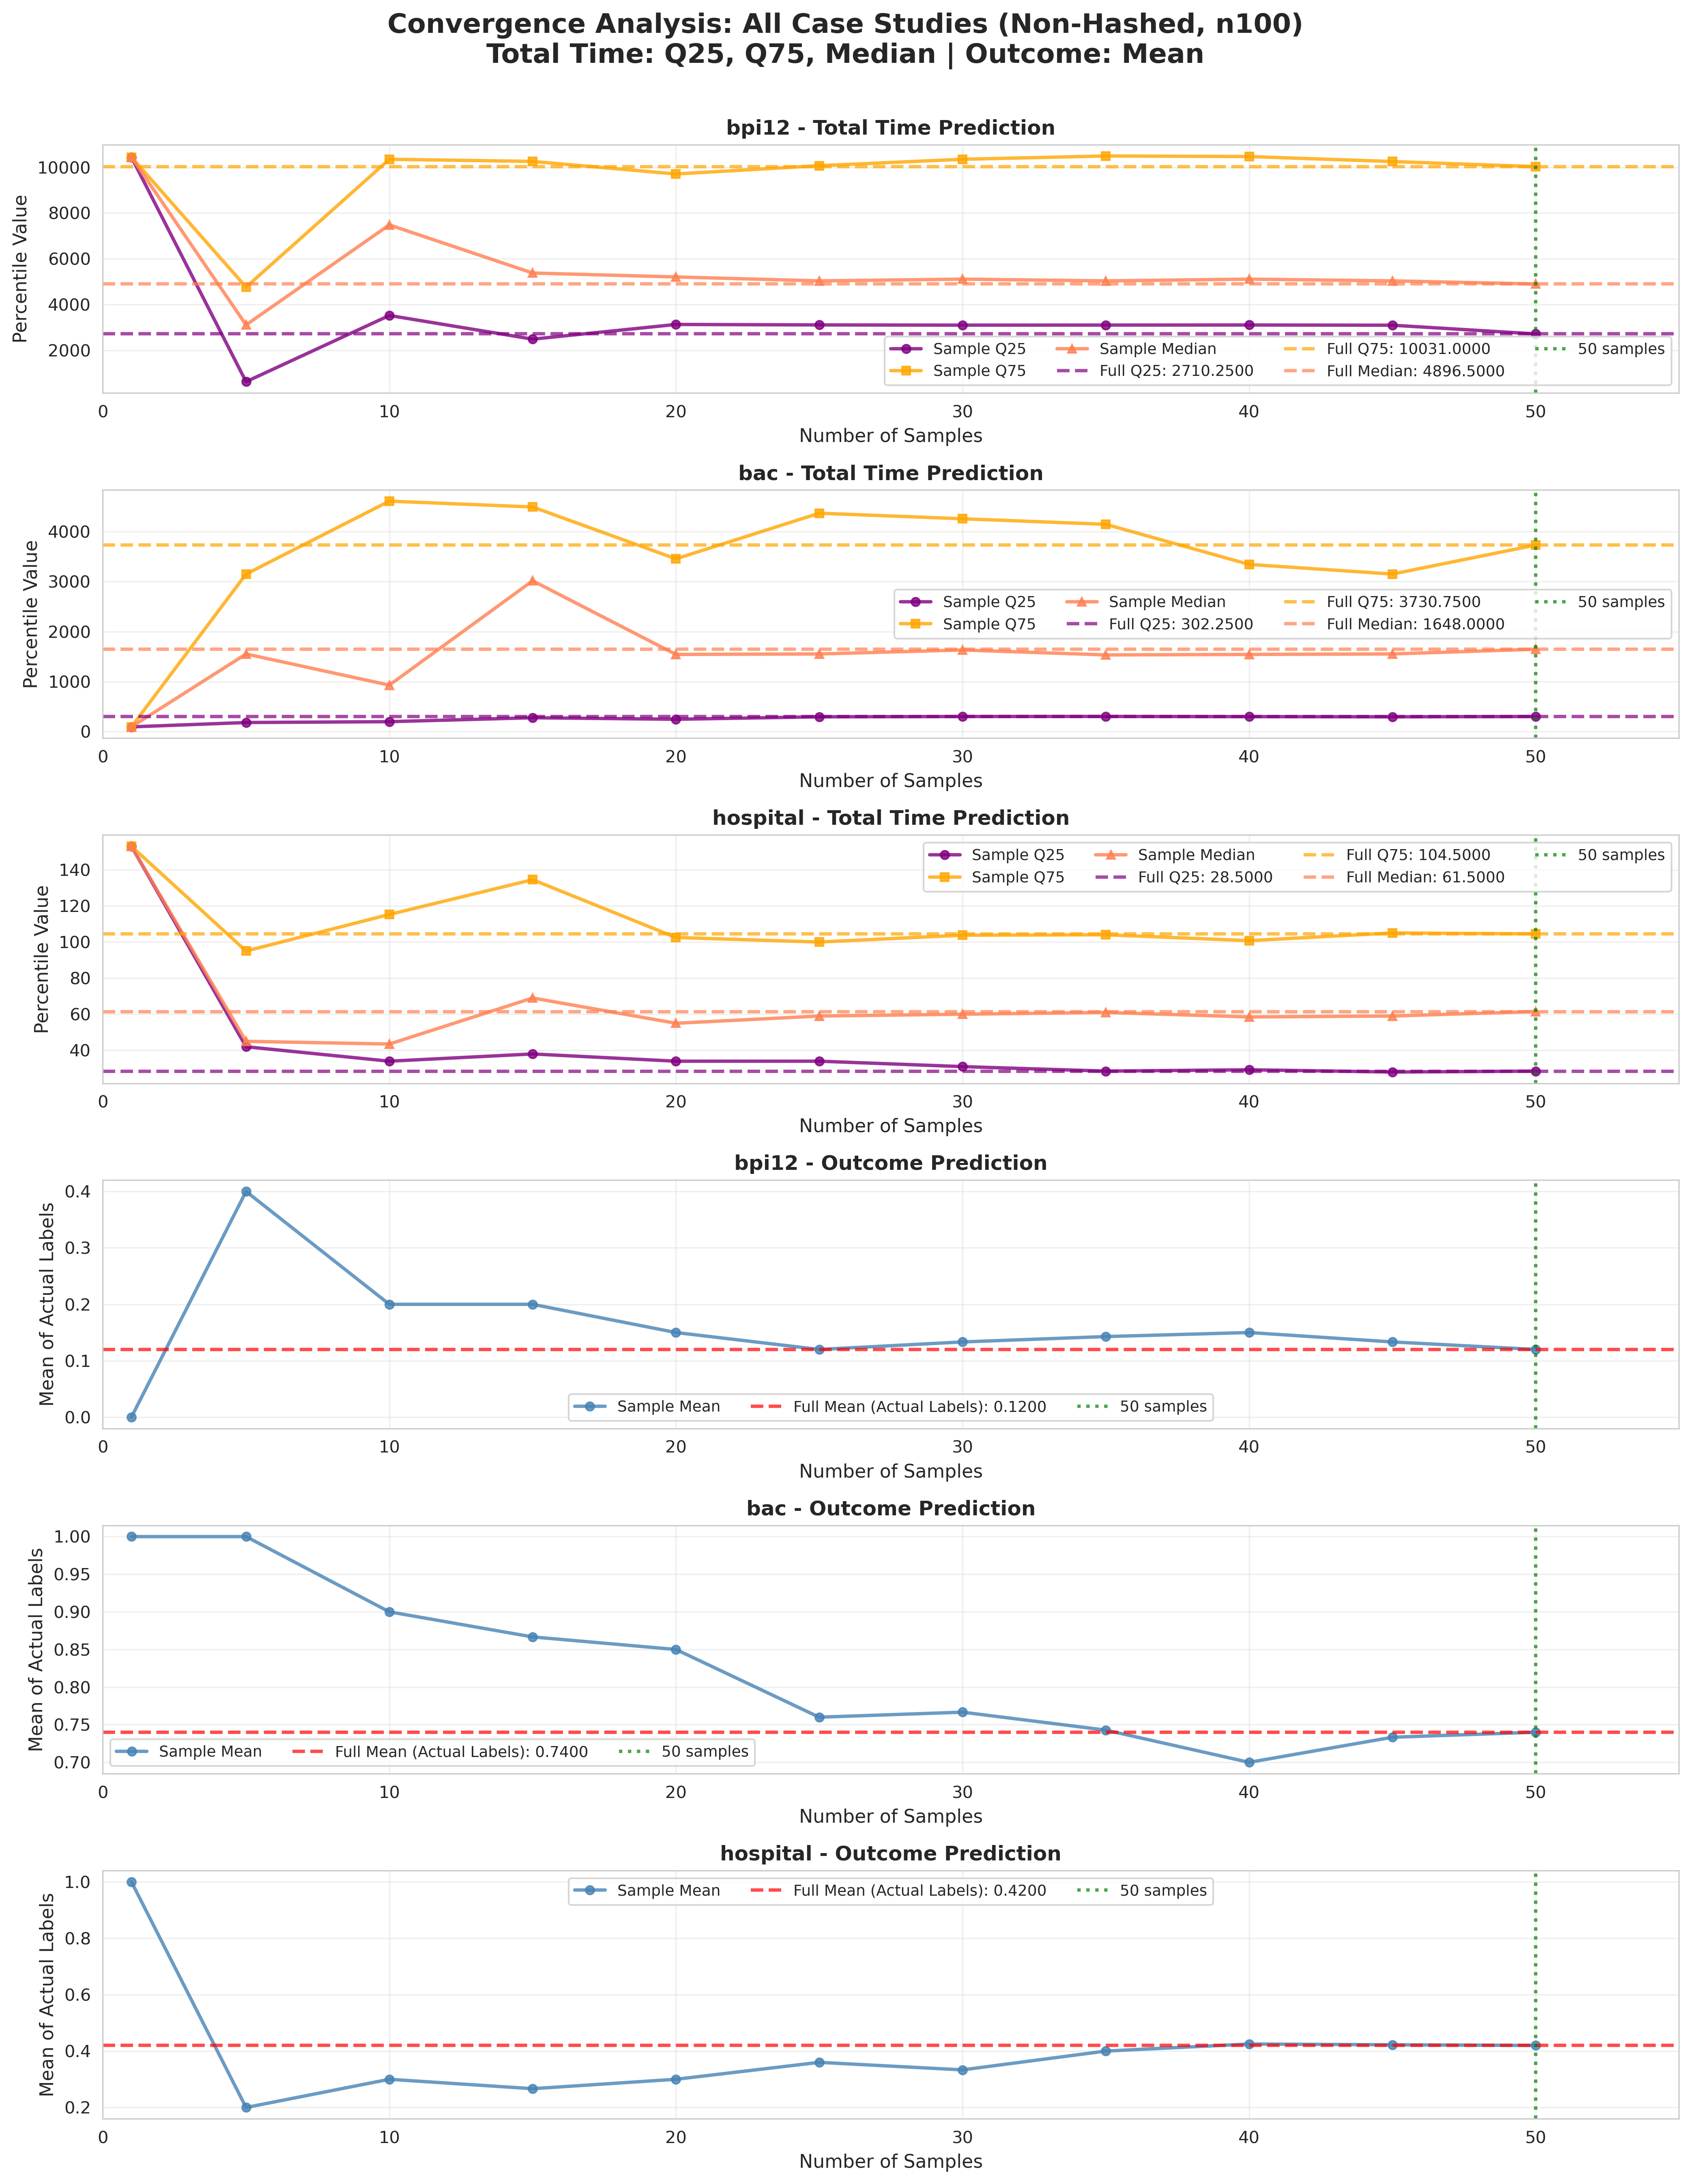
\includegraphics[width=.90\linewidth]{Figs/quartile_convergence_all.png}
\label{fig:convergence}
\Description{Placeholder}
\end{figure}

Finally, Table~\ref{tab:good_turing_all} provides results in terms of \textit{the probability of encountering a new $\beta$-learner} when analyzing other 1, 10 or 100 LLM's outputs. Strong empirical evidence supporting the claim that the probability of discovering novel $\beta$-learner patterns in future predictions approaches zero. Expected novel $\beta$-learners for $m=1,10,100$ additional traces approach zero in every use case and KPI. Specifically, after 1 new running trace, the probability is exactly 0 for both KPI of total time and activity occurrence. After 10 new running traces, it rises to 0.1\% and 0.4\% for respectively total time and activity occurrence, reaching 0.3\% and 1.4\% after 100 new running traces.


Furthermore, Figure~\ref{fig:convergence} plots the convergence curves of the different KPI distributions (total time on top rows and activity occurrence on bottom rows) when analyzing a given number of traces, also divided per use case. From the different plots it is possible to visualize that the convergence in the distribution has already been reached after roughly 30 traces.


\section{Conclusion}\label{sec:concl}
This paper advances our previous work~\cite{10.1007/978-3-032-02929-4_16} in the field of Predictive Process Monitoring in data-scarce environments through a comprehensive LLM prompting framework. It addresses three new research questions via empirical analysis across three real public and private event logs and two different Key Performance Indicators.

RQ1 confirms the LLM's superiority when the model can only leverage 100 traces as training, outperforming state-of-the-art benchmarks for both KPIs. This demonstrates that the LLM is a viable alternative for implementing Predictive Process Monitoring frameworks, especially in scenarios where data availability is limited.

RQ2 empirically proves semantic leverage: the context in the prompts was hashed and the experiments repeated, showing that the LLM exploits its embodied knowledge to provide predictions for running traces. The results were also statistically verified using the Nemenyi post-hoc test.

RQ3 reveals the reasoning anatomy: manual inspection of 50 traces for each use case and KPI led to the identification of various predictors that the LLM employs, the so-called $\beta$-learners. These have been shown to include all possible ones through Good-Turing validation. This paper demonstrates not only that the LLM outperforms every model it mimics but also that it performs more complex analyses than those models, cherry picking outliers to remove.

Future work will focus on exploring new LLMs, given the rapid evolution of the field, and will include user studies on the reliance on $\beta$-learners, longer context length, also deriving more complex learners. Another direction is to extend this work toward a Prescriptive Process Analytics framework, enabling not only predictions but also actionable recommendations derived from the predictions. Finally, this should be extended to prediction on Object-Centric-Event-Logs~\cite{DBLP:conf/adbis/GhahfarokhiPBA21,DBLP:conf/bpm/LeoniV25}, where events can relate to multiple objects of different types, unlike traditional case-centric logs that assume one event per case.



% \section{Before Submitting}

% \subsection{Blind Your Manuscript}

% \subsection{Select Your Department}

% \subsection{What to Submit}


\newpage

\bibliographystyle{ACM-Reference-Format}

\bibliography{bibliography}

\pagebreak

\pagebreak




\section*{Appendix}\label{sec:appendix}

In this Section is reported an example of an hashed input prompt for the KPI of total time prediction, with its corresponding answer returned from the LLM.

\lstset{
basicstyle=\fontsize{6.1}{8}\ttfamily,
    label={lst:hashed_ao},
    numbers=left,
    caption={Prompting technique example for a loan application process (Bpi12), for the KPI of Activity Occurrence. In the example, only 2 training traces are provided due to space limitation.},
    captionpos=b,
    moredelim=**[is][\bfseries]{@}{@},
    float=t
} % Adjust scale as needed
\begin{lstlisting}
You are a process mining expert. Your task is to predict the occurrence of the activity 
"4DNF" that is likely to occur in a running process instance based on complete ones.

Each trace is mapped as a sequence of activities and integers representing the minutes since the start of the process. 
The log is represented as a python list containing one dictionary for each trace. Included in it are:

- the key "5U8T" where the value represents the value of a global variable.
- the key "ActTimeSeq", which value is a list of [activity, cumulative elapsed minutes] 

All interactions will be structured in the following way, with the appropriate values filled in.

[[ ## reasoning ## ]]
{your step-by-step reasoning}

[[ ## answer ## ]]
{your predicted occurrence of 5U8T that has to be either 0 or 1 as an integer}

[[ ## completed ## ]]

In adhering to this structure, your objective is to analyze the event log, and apply reasoning to derive the occurrence
of 4DNF for a new case that is not completed yet. 
Ensure to articulate each step of your thought process in the reasoning field, detailing how you identify relationships 
with past cases and leverage your intuition about the meaning of activities to arrive at the solution. 
The `answer` should be the final prediction of the occurrence of 4DNF for the given process instance.

Respond with the corresponding output fields, starting with the field [[ ## reasoning ## ]], 
then [[ ## answer ## ]], and then ending with the marker for [[ ## completed ## ]].

The following table shows some example cases with their associated occurrence of 4DNF:

{"5U8T": 5000.0, "ActTimeSeq": [["URXY", 11], ["4DNF", 1464], ["4DNF", 7486]]}
{"5U8T": 15000.0, "ActTimeSeq": [["URXY", 13], ["4DNF", 14], ["5GH2", 4328], ["5GH2", 8792]]}
... 
... 
    
Now predict the total time for this new uncompleted case, considering that the case is still running:

{"Application_1000386745": {"5U8T": 18000.0, "ActTimeSeq": [["URXY", 2], ["4DNF", 8571], ["Running"]]}

Now predict the occurrence of 4DNF for this new case:\n\n{test_case}"

\end{lstlisting}%\label{lst:hashed_ao}
\lstset{basicstyle=\fontsize{6.1}{8}\ttfamily, label={lst:hashed_ao_answ},
caption={Output prompt for the prompt in~\ref{lst:hashed_ao}.},
captionpos=b, float=tb} % Adjust scale as needed
\begin{lstlisting}
The objective is to predict whether the activity "4DNF" will occur in the given incomplete trace. 

I will analyze the provided completed traces to identify patterns and conditions associated with the occurrence of "4DNF". 

[[ ## reasoning ## ]]
1. **Analyze traces where "4DNF" occurred (4DNF = 1):** 
* I observed that in all traces where "4DNF" occurs, the activity "URXY" always precedes the first occurrence of "4DNF". 
For example: * `{"ActTimeSeq": [... "URXY", 10199], ["4DNF", 10201] ...}` * `{"ActTimeSeq": [... "URXY", 21577], 
["4DNF", 21591] ...}` * `{"ActTimeSeq": [... "URXY", 24034], ["4DNF", 24265] ...}` * This establishes a strong dependency: 
"URXY" must happen before "4DNF". 
* Furthermore, these "4DNF=1" traces typically follow a sequence like `DNZ0` -> `G1ZM` (multiple) -> `URXY` -> `4DNF`. 

2. **Analyze traces where "4DNF" did not occur (4DNF = 0):** * Many traces do not contain "4DNF". 
* Specifically, there are cases that contain `DNZ0` and `G1ZM` but *no* `URXY` and consequently no `4DNF`. For example: 
* `{"5U8T": "7800", "ActTimeSeq": [["YC7U", 2], ["DNZ0", 4], ["G1ZM", 10180], ["G1ZM", 12921]], "4DNF": 0}` * 
`{"5U8T": "80000", "ActTimeSeq": [["DNZ0", 12], ["G1ZM", 10638]], "4DNF": 0}` * There are also cases where `URXY` occurs, 
but `4DNF` does not. In these scenarios, `URXY` is typically the last activity in the trace, indicating the process completed 
before `4DNF` could be triggered. 

3. **Evaluate the new, incomplete case:** 
* The new case is `{"5U8T": "10000", "ActTimeSeq": [["DNZ0", 1], ["DNZ0", 165], ["DNZ0", 253], ["G1ZM", 255]]}`. 
* The sequence of activities in this case is `DNZ0` (multiple times) followed by `G1ZM`. 
* Crucially, the activity `URXY` has not yet occurred in this trace. 

4. **Conclusion:** * Since "URXY" is a prerequisite for "4DNF" in all observed cases where "4DNF" eventually occurs, 
and "URXY" has not yet been observed in the current trace, it is highly unlikely that "4DNF" will occur at this stage
or as the next activity. The process needs to progress further (specifically, to include "URXY") before "4DNF" 
can be considered.

[[ ## answer ## ]]
0
[[ ## completed ## ]]


\end{lstlisting}













\end{document}
\endinput
%%
%% End of file `sample-manuscript.tex'.
